% !TeX program = xelatex
% !TeX encoding = UTF-8
% !TeX root = document.tex

% Command to compile document
% xelatex -synctex=1 -interaction=nonstopmode document.tex

% Recomended IDE is TeXstudio (https://texstudio.org/) 
% or another one, that supports magic comments

% Document class repo 
% https://github.com/mirea-ninja/Latex-Template-for-Report-Diploma-Thesis/

\documentclass{mirea}

\usepackage{array}
\usepackage{longtable}
\usepackage{float}


\usepackage{hyperref}
\hypersetup{pdftitle={Курсовая работа 5 семестр}, pdfauthor={В. С. Верхотуров}}

\usepackage{graphicx}

\begin{document}
	
	\begin{titlepage}
		
		\pagestyle{empty}
		
		\vspace*{-1.5cm}
		\hspace*{-3.2cm}
		
\includegraphics[height=.89\paperheight]{titlepage.jpeg}
		\newpage
		
		\setlength\parindent{0pt}
		\newcommand{\blankDate}[2]{\mbox{\uline{<<\makebox[.7cm]{#1}>>~\makebox[2cm]{#2}~\the\year{}~г.}}} % {день}{месяц}
		\newcommand\blankLine[2]{$\underset{\text{#1}}{\text{\uline{#2}}}$}
		\begin{center}
			\includegraphics[width=2.5cm]{MIREA_Gerb_Black} \par
			МИНОБРНАУКИ РОССИИ \par 
			Федеральное государственное бюджетное образовательное учреждение высшего образования \par
			\textbf{<<МИРЭА~--- Российский технологический университет>>} \par
			\textbf{\fontsize{16pt}{16pt}\selectfont РТУ МИРЭА} \par
			\blankLine{(наименование института, филиала)}{Институт кибербезопасности и цифровых технологий} \par
			\blankLine{(наименование кафедры)}{Кафедра КБ-14 <<Цифровые технологии обработки данных>>} \par
			\vspace*{1cm}
			{\fontsize{16pt}{16pt}\selectfont
				\textbf{КУРСОВОЙ ПРОЕКТ (РАБОТА)}} \par
			по дисциплине \blankLine{(наименование дисциплины)}{Программные средства манипулирования данными}
		\end{center}
		\textbf{Тема курсовой работы \uline{Проектирование баз данных}} \bigskip\par
		Студент группы \blankLine{учебная группа, фамилия, имя, отчество студента}{БСБО-05-20 В.~С.~Верхотуров} \hfill\blankLine{подпись студента}{\hspace{4cm}} \bigskip\par
		Руководитель курсовой работы \blankLine{}{И.\,А.\,Иванова} \hfill\blankLine{подпись руководителя}{\hspace{4cm}} \bigskip\par
		Член комиссии \blankLine{}{И.\,Д.\,Котилевец} \hfill\blankLine{подпись члена комиссии}{\hspace{4cm}} \bigskip\par
		\begin{tabular}{@{}ll}
			Работа предоставлена к защите & \blankDate{}{} \bigskip\\
			Допущен к защите & \blankDate{}{}
		\end{tabular}
		\begin{center}
			\vfill Москва~--- \the\year{}~г.
		\end{center}
	
		\newpage
		\begin{center}
			\includegraphics[width=2.5cm]{MIREA_Gerb_Black} \par
			МИНОБРНАУКИ РОССИИ \par 
			Федеральное государственное бюджетное образовательное учреждение высшего образования \par
			\textbf{<<МИРЭА~--- Российский технологический университет>>} \par
		\end{center}
		
		Институт ИКЦТ направление \underline{09.03.02 <<Информационные системы и технологии>>}
		
		Кафедра КБ-4 <<Интеллектуальные системы информационной безопасности>>
		
		Дисциплина \underline{<<Программные средства манипулирования данными>>}
		
		\begin{center}
			\vspace*{1cm}
			{\fontsize{16pt}{16pt}\selectfont
				\textbf{ПОЯСНИТЕЛЬНАЯ ЗАПИСКА \\ к курсовой работе (проекту) }} \par
		\end{center}
	
		Студент \underline{В.\,C.\,Верхотуров} \par\vspace*{.3cm}
		Группа \underline{БСБО-05-20} \par\vspace*{.3cm}
		Работа защищена на оценку \underline{\hspace*{5cm}} \par\vspace*{.3cm}
		Руководитель работы	\underline{И.\,А.\,Иванова} \par\vspace*{.3cm}
		Член комиссии \underline{И.\,Д.\,Котилевец}
		\begin{center}
			\vfill Москва~--- \the\year{}~г.
		\end{center}
	
		\newpage
		\begin{center}
			\includegraphics[width=2.5cm]{MIREA_Gerb_Black} \par
			МИНОБРНАУКИ РОССИИ \par 
			Федеральное государственное бюджетное образовательное учреждение высшего образования \par
			\textbf{<<МИРЭА~--- Российский технологический университет>>} \par
		\end{center}
	
		Институт ИКЦТ направление \underline{09.03.02 <<Информационные системы и технологии>>}
		
		Кафедра КБ-4 <<Интеллектуальные системы информационной безопасности>>
		
		Дисциплина \underline{<<Программные средства манипулирования данными>>}
		
		\begin{center}
			\vspace*{1cm}
			{\fontsize{16pt}{16pt}\selectfont
				\textbf{ЗАДАНИЕ НА КУРСОВУЮ РАБОТУ}} \par
		\end{center}
	
		Студент 3 курса группы БСБО-05-20.
		
		\begin{enumerate}
			\item Тема: Проектирование баз данных
			\item Срок представления проекта (работы) к защите: 23.12.2022
			\item Содержание пояснительной записки:
			\begin{itemize}
				\item Задание
				\item Содержание
				\item Описание предметной области
				\item Список использованных источников
				\item Приложения
			\end{itemize}
		\end{enumerate}
	
		Руководитель работы \underline{И.\,А.\,Иванова}
		
		Задание принял к исполнению \underline{И.\,Д.\,Котилевец}
		
		\begin{center}
			\vfill Москва~--- \the\year{}~г.
		\end{center}
	\end{titlepage}
	\addtocounter{page}{3}
	
	
	\tableofcontents
	
	\section*{Задание}
	\phantomsection
	\addcontentsline{toc}{section}{Задание}
	
	В данной работе необходимо разработать базу данных для агрегатора новостей РТУ МИРЭА, подключить CMS Strapi, создать пользовательский веб интерфейс на React для пользователей агрегатора.
	
	В заключении работы требуется подготовить полную документацию проекта, включая код программы и скриншоты работы приложения.
	
	
	\section*{Введение}
	\phantomsection
	\addcontentsline{toc}{section}{Введение}
	
	Целью данного курсового проекта является разработка базы данных для автоматизации работы агрегатора новостей РТУ МИРЭА.
	
	Задачей данного проекта является разработка базы данных для централизованного хранения данных агрегатора и для автоматизации работы агрегатора, также требуется разработать веб-интерфейс для того, чтобы сделать процесс взаимодействия с системой доступнее
	
	
	\section{ER-модель предметной области}
	
	ER–модель предметной области указана на рисунке \ref{fig:er}.
	
	\begin{figure}[H]
		\centering
		%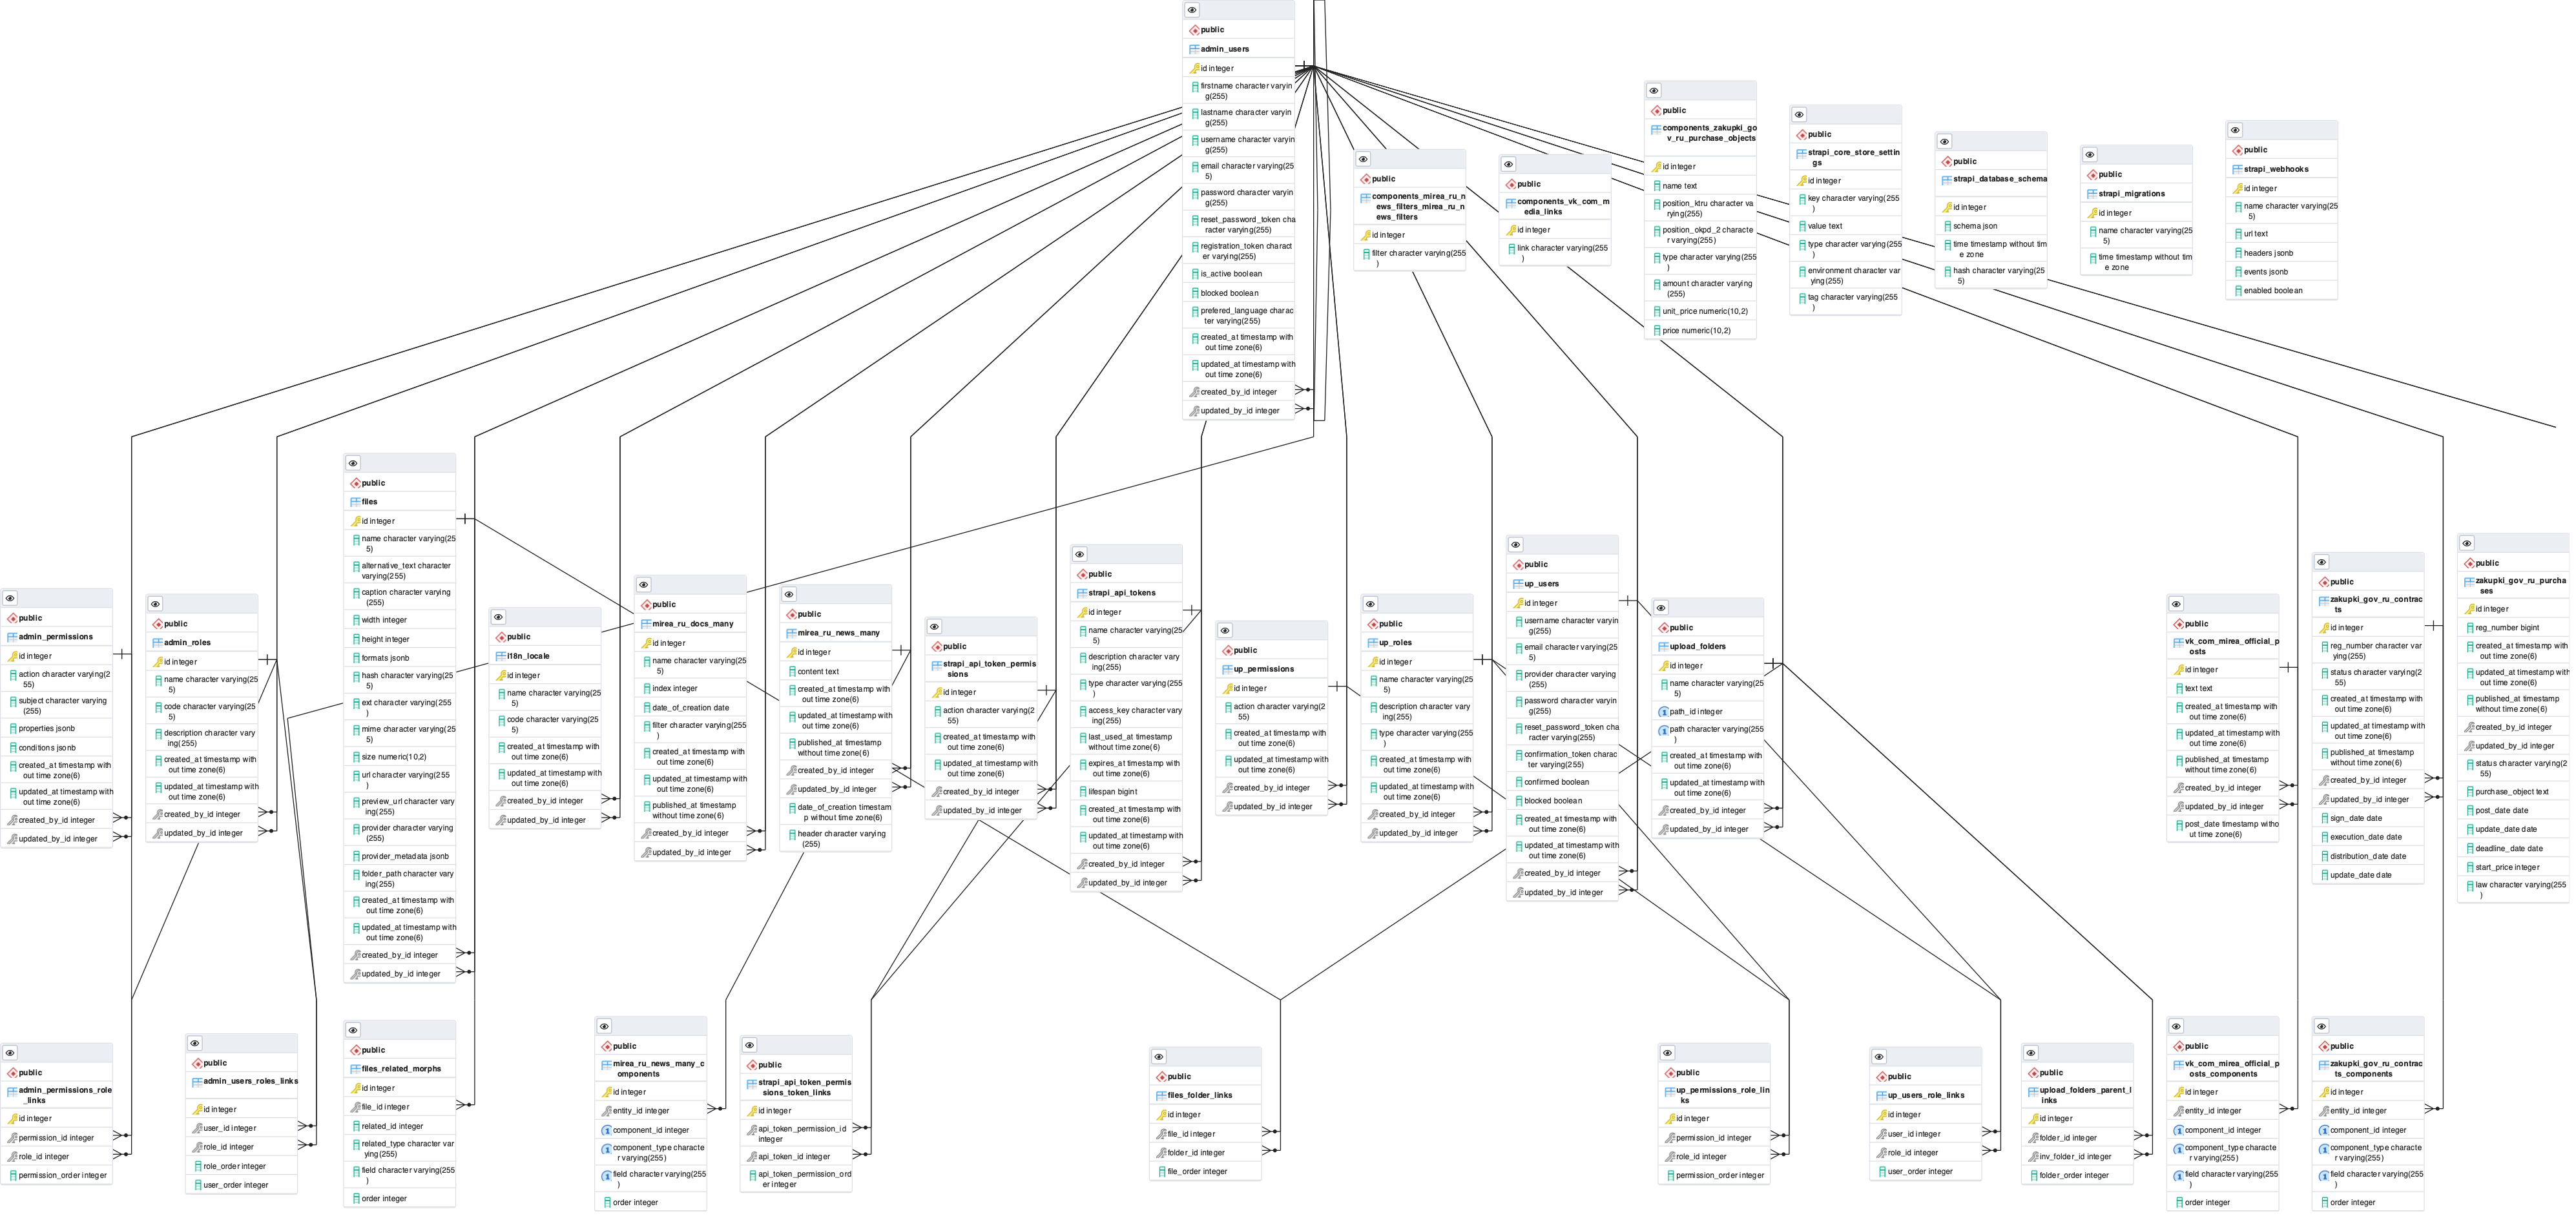
\includegraphics[width=.7\textheight, height=.85\textwidth, angle=90]{er}
		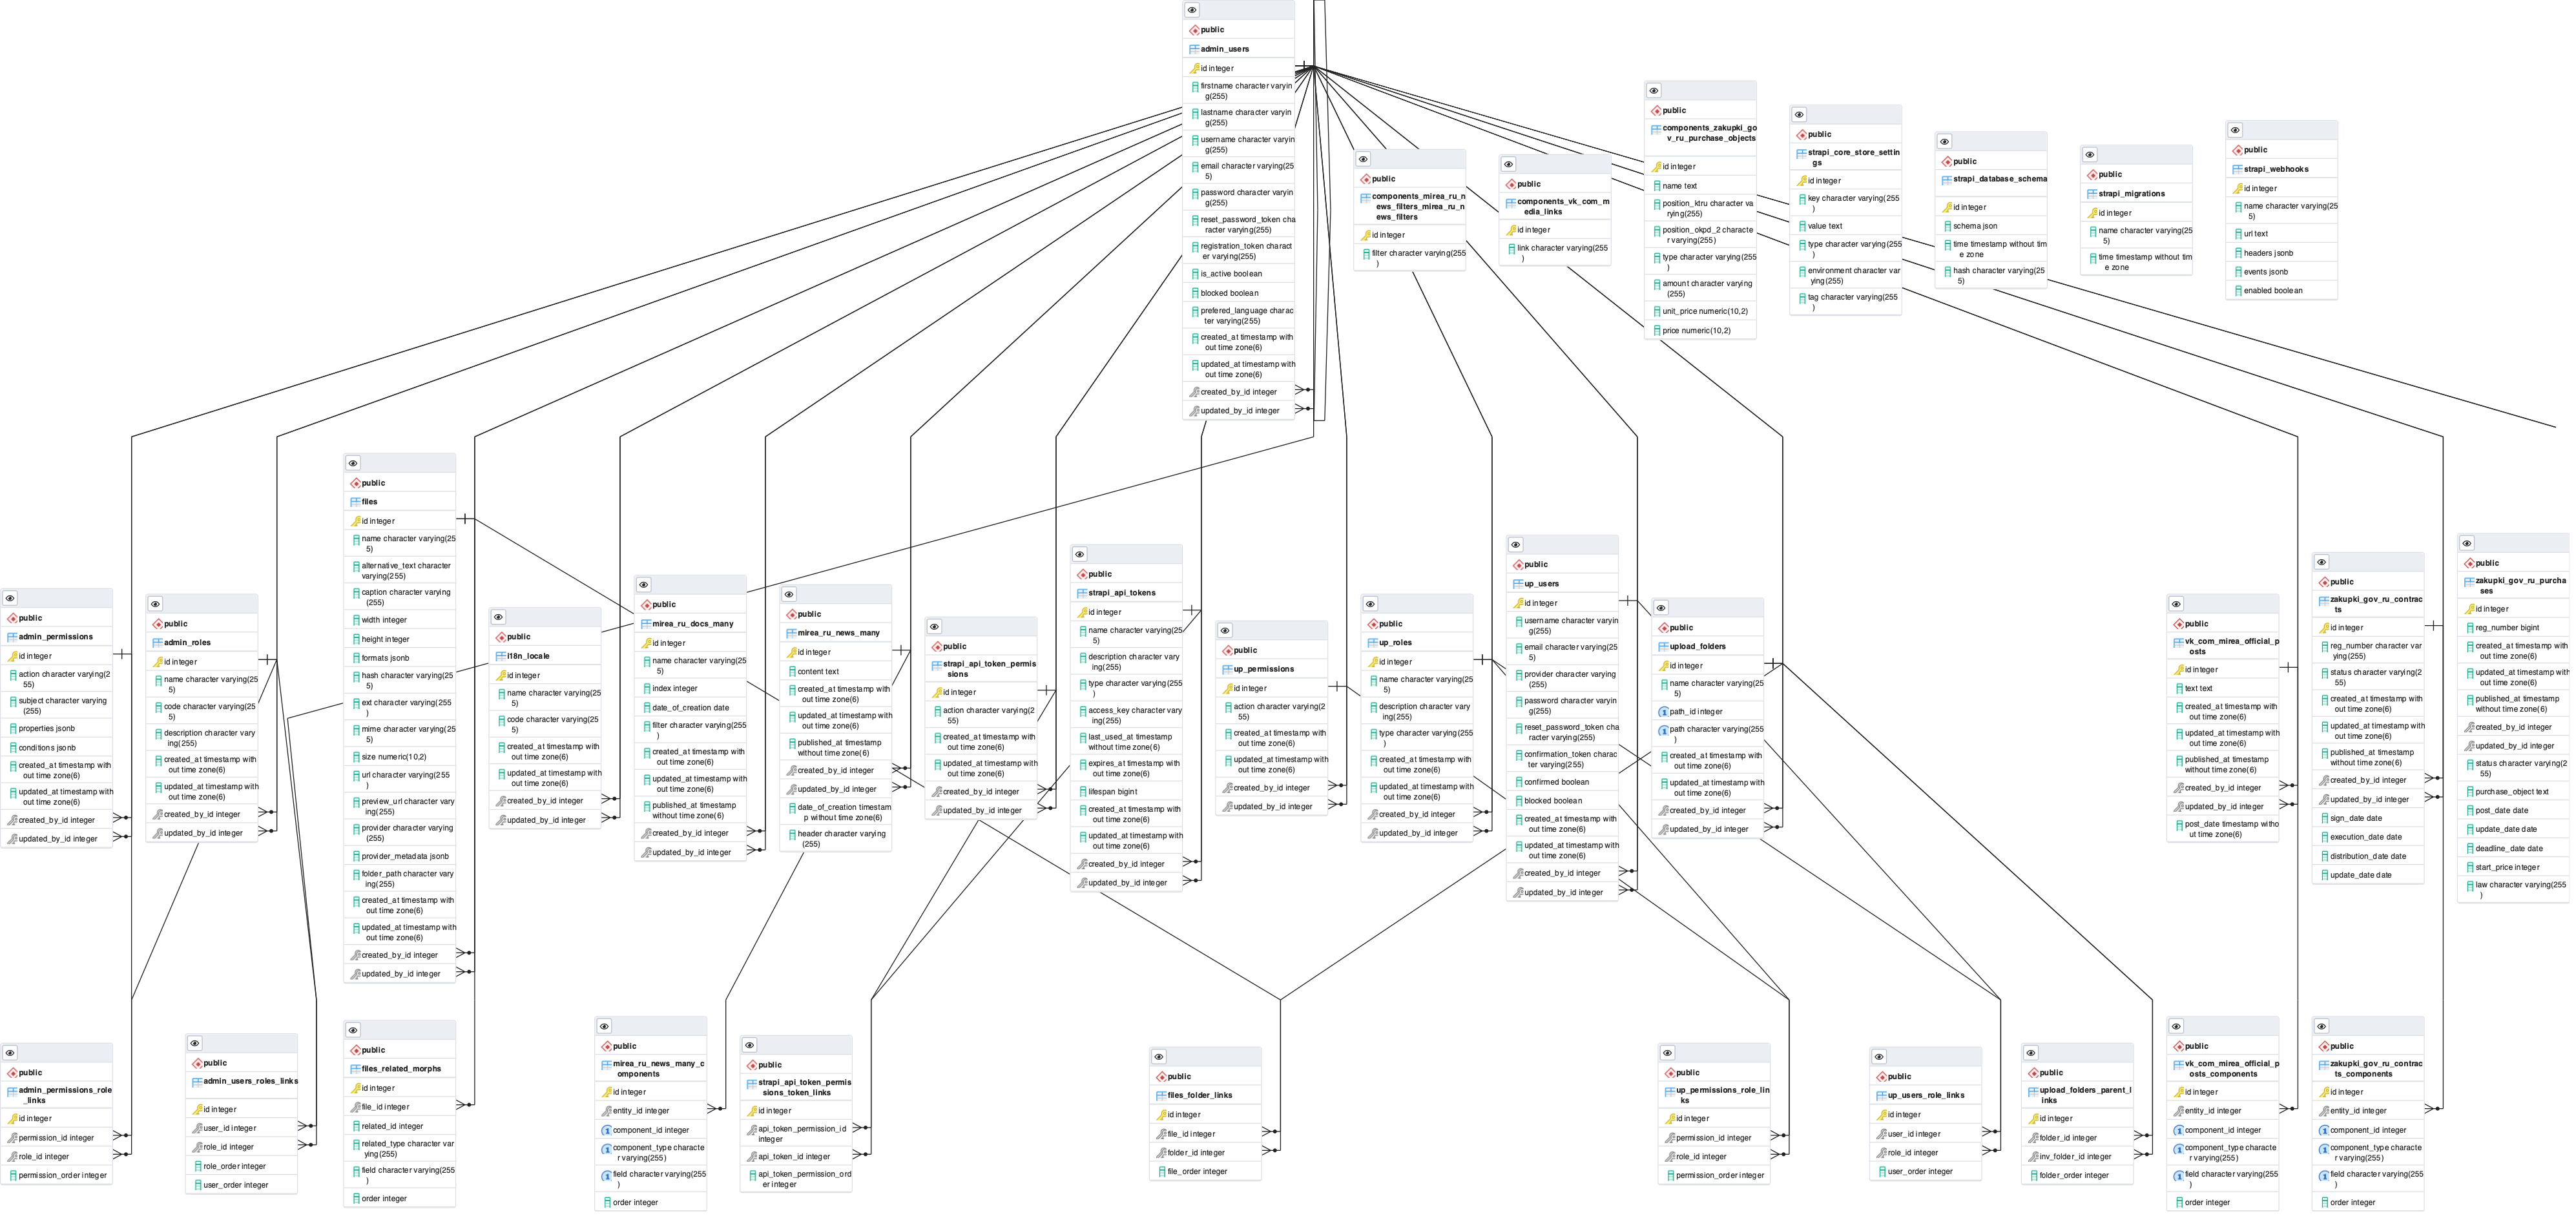
\includegraphics[width=\textwidth]{er}
		\parskip=6pt
		\caption{ER-модель}
		\label{fig:er}
	\end{figure}
	
	\subsection{Сущности}
	
	В таблице~\ref{tab:enities} приведено описание сущностей спроектированной базы
	данных.
	
	\begin{longtable}{ |p{.4\textwidth} |p{.25\textwidth} |p{.05\textwidth} |p{.2\textwidth}| } 
		\caption{Сущности спроектированной БД}
		\label{tab:enities}
		\endfirsthead
		\endhead
		\hline
		\textbf{Название таблицы} & \textbf{Назначение} & \textbf{Пер\-вич\-ный ключ} & \textbf{Вторичный ключ} \\ \hline
		
		admin\_permissions & Все доступные разрешения пользователей в админ панели & id & created\_by\_id, updated\_by\_id \\ \hline 
		
		admin\-\_permissions\-\_role\-\_links & Связь ролей и разрешений & id & permission\_id, role\_id \\ \hline 
		
		admin\-\_roles & Роли в админ панели & id & created\_by\_id, updated\_by\_id \\ \hline
		
		admin\-\_users & Пользователи админ панели & id & created\_by\_id, updated\_by\_id \\ \hline
		
		admin\-\_users\-\_roles\-\_links & Связь пользователя с ролью & id & user\_id, role\_id \\ \hline
		
		components\-\_mirea\-\_ru\-\_news\-\_filters\-\_mirea\-\_ru\-\_news\-\_filters & Классификатор фильтров новостей & id & \\ \hline
		
		components\-\_vk\-\_com\-\_media\-\_links & Ссылки на прикрепленные медиа файлы ВК новостей & id & \\ \hline
		
		components\-\_zakupki\-\_gov\-\_ru\-\_purchase\-\_objects & Объекты закупки контракта & id & \\ \hline
		
		files & Метадата файлов, пути, по котором можно найти файлы & id & created\_by\_id, updated\_by\_id \\ \hline
		
		files\_folder\_links & Файлы можно сгруппировать по директориям & id & file\_id, folder\_id \\ \hline
		
		files\_related\_morphs & Связь файла с кортежем в пользовательской таблице & id & file\_id, related\_id \\ \hline
		
		i18n\_locale & Доступные локализации & id & created\_by\_id, updated\_by\_id \\ \hline
		
		mirea\_ru\_docs\_many & Новости о документах & id & created\_by\_id, updated\_by\_id \\ \hline
		
		mirea\_ru\_news\_many & Новости МИРЭА на сайте & id & created\_by\_id, updated\_by\_id \\ \hline
		
		mirea\_ru\_news\_many\-\_components & Связь новости МИРЭА на сайте и фильтров & id & entity\_id, component\_id \\ \hline
		
		strapi\_api\_token\_permissions & Разрешения для пользователей, авторизирующихся по токену & id & created\_by\_id, updated\_by\_id \\ \hline
		
		strapi\_api\_token\_permissions\-\_token\_links & Связь токенов и разрешений & id & api\_token\-\_permission\_id, api\_token\_id \\ \hline
		
		strapi\_api\_tokens & Выданные токены & id & created\_by\_id, updated\_by\_id \\ \hline
		
		strapi\_core\_store\_settings & Настройки админ панели, плагинов & id & \\ \hline
		
		strapi\_database\_schema & Схема БД в JSON & id & \\ \hline
		
		strapi\_migrations & Миграции БД & id & \\ \hline
		
		strapi\_webhooks & Вебхуки CMS & id & \\ \hline
		
		up\_permissions & Разрешения для клиентов & id & created\_by\_id, updated\_by\_id \\ \hline
		
		up\_permissions\_role\_links & Связь разрешений и ролей клиентов & id & permission\_id, role\_id \\ \hline
		
		up\_roles & Роли клиентов & id & created\_by\_id, updated\_by\_id \\ \hline
		
		up\_users & Клиенты & id & created\_by\_id, updated\_by\_id \\ \hline
		
		up\_users\_role\_links & Связь ролей с клиентами & id & user\_id, role\_id \\ \hline
		
		upload\_folders & Директории для файлов & id & created\_by\_id, updated\_by\_id \\ \hline
		
		upload\_folders\_parent\_links & Иерархия директорий & id & folder\_id, inv\_folder\_id \\ \hline
		
		vk\_com\_mirea\_official\_posts & Новости из ВК постов & id & created\_by\_id, updated\_by\_id \\ \hline
		
		vk\_com\_mirea\-\_official\-\_posts\-\_components & Связь ВК постов с компонентом медиа ссылок & id & entity\_id, component\_id \\ \hline
		
		zakupki\_gov\_ru\_contracts & Контракты МИРЭА & id & created\_by\_id, updated\_by\_id \\ \hline
		
		zakupki\_gov\_ru\-\_contracts\-\_components & Связь контрактов и объектов закупки & id & entity\_id, component\_id \\ \hline
		
		zakupki\_gov\_ru\_purchases & Закупки & id & entity\_id, component\_id \\ \hline
		
	\end{longtable}


	\subsection{Атрибуты}
	
	В таблицах \ref{tab:attributes_first_table}-\ref{tab:attributes_last_table} приведено описание атрибутов каждой сущности.
	
	\begin{longtable}{ |p{.25\textwidth}|p{.25\textwidth}|p{.2\textwidth}|p{.2\textwidth}| } 
		\caption{Описание атрибутов сущности admin\_permissions}
		\label{tab:attributes_first_table}
		\endfirsthead
		\endhead
		\hline
		Наименование атрибута & Назначение атрибута & Тип & Примечание \\ \hline
		
		id & Идентификацион\-ный номер разрешения пользователя админ панели & integer & Первичный ключ, уникальное поле \\ \hline
		
		action & Название разрешения & character varying (255) & Пример: plugin::content-manager.explorer.\-create \\ \hline
		
		subject & Таблица, для которой действует разрешение  & character varying (255) & Пример: api::vk-com-mirea-official-post.vk-com-mirea-official-post \\ \hline
		
		properties & Доступные колонки  & jsonb & \\ \hline
		
		condition & Доп условия предоставления разрешения & jsonb & \\ \hline
		
		created\_at & Время создания кортежа & timestamp(6) without time zone & \\ \hline
		
		updated\_at & Время обновления кортежа & timestamp(6) without time zone & \\ \hline
		
		created\_by\_id & Пользователь, создавший кортеж & integer & Внешний ключ \\ \hline
		
		updated\_by\_id & Пользователь, создавший кортеж & integer & Внешний ключ \\ \hline
		
	\end{longtable}

	\begin{longtable}{ |p{.25\textwidth}|p{.25\textwidth}|p{.2\textwidth}|p{.2\textwidth}| } 
		\caption{Описание атрибутов сущности admin\_permissions\_role\_links}
		\endfirsthead
		\endhead
		\hline
		Наименование атрибута & Назначение атрибута & Тип & Примечание \\ \hline
		
		id & Идентификацион\-ный номер связи & integer & Первичный ключ, уникальное поле \\ \hline
		
		permission\_id & Идентификационный номер разрешения & integer & Внешний ключ \\ \hline
		
		role\_id & Идентификационный номер роли & integer & Внешний ключ \\ \hline
		
		permission\_order & Порядок отображения в UI & integer & \\ \hline
		
	\end{longtable}

	\begin{longtable}{ |p{.25\textwidth}|p{.25\textwidth}|p{.2\textwidth}|p{.2\textwidth}| } 
		\caption{Описание атрибутов сущности admin\_roles}
		\endfirsthead
		\endhead
		\hline
		Наименование атрибута & Назначение атрибута & Тип & Примечание \\ \hline
		
		id & Идентификацион\-ный номер роли админ панели & integer & Первичный ключ, уникальное поле \\ \hline
		
		name & Название роли & character varying (255) & Задается администратором \\ \hline
		
		code & Название, генерирующееся втоматически  & character varying (255) & Уникальное поле \\ \hline
		
		description & Описание роли  & character varying (255) & \\ \hline
		
		created\_at & Время создания кортежа & timestamp(6) without time zone & \\ \hline
		
		updated\_at & Время обновления кортежа & timestamp(6) without time zone & \\ \hline
		
		created\_by\_id & Пользователь, создавший кортеж & integer & Внешний ключ \\ \hline
		
		updated\_by\_id & Пользователь, создавший кортеж & integer & Внешний ключ \\ \hline
		
	\end{longtable}

	\begin{longtable}{ |p{.25\textwidth}|p{.25\textwidth}|p{.2\textwidth}|p{.2\textwidth}| } 
		\caption{Описание атрибутов сущности admin\_users}
		\endfirsthead
		\endhead
		\hline
		Наименование атрибута & Назначение атрибута & Тип & Примечание \\ \hline
		
		id & Идентификацион\-ный номер пользователя админ панели & integer & Первичный ключ, уникальное поле \\ \hline
		
		firstname & Имя пользователя & character varying (255) & Задается пользователем при регистрации \\ \hline
		
		lastname & Фамилия пользователя & character varying (255) & Задается пользователем при регистрации \\ \hline
		
		username & Ник пользователя & character varying (255) & Задается пользователем при регистрации \\ \hline
		
		email & Фамилия пользователя & character varying (255) & Проверка на валидность по регулярному выражению \\ \hline
		
		password & Пароль & character varying (255) & Хэшированный с солью \\ \hline
		
		reset\_password\_token & Токен изменения пароля & character varying (255) & Возможность CMS, не используется \\ \hline
		
		registration\_token & Токен приглашения зарегистрироваться & character varying (255) & Возможность CMS, приглашение редакторов \\ \hline
		
		is\_active & Учетная запись не просрочена & boolean & \\ \hline
		
		blocked & Учетная запись заблокирована администратором & boolean & \\ \hline
		
		prefered\_language & Язык интерфейса & character varying (255) & \\ \hline
		
		created\_at & Время создания кортежа & timestamp(6) without time zone & \\ \hline
		
		updated\_at & Время обновления кортежа & timestamp(6) without time zone & \\ \hline
		
		created\_by\_id & Пользователь, создавший кортеж & integer & Внешний ключ \\ \hline
		
		updated\_by\_id & Пользователь, создавший кортеж & integer & Внешний ключ \\ \hline
		
	\end{longtable}

	\begin{longtable}{ |p{.25\textwidth}|p{.25\textwidth}|p{.2\textwidth}|p{.2\textwidth}| } 
		\caption{Описание атрибутов сущности admin\_users\_roles\_links}
		\endfirsthead
		\endhead
		\hline
		Наименование атрибута & Назначение атрибута & Тип & Примечание \\ \hline
		
		id & Идентификацион\-ный номер связи & integer & Первичный ключ, уникальное поле \\ \hline
		
		user\_id & Идентификационный номер пользователя & integer & Внешний ключ \\ \hline
		
		role\_id & Идентификационный номер роли & integer & Внешний ключ \\ \hline
		
		role\_order & Порядок отображения в UI & integer & \\ \hline
		
		user\_order & Порядок отображения в UI & integer & \\ \hline
		
	\end{longtable}

	\begin{longtable}{ |p{.25\textwidth}|p{.25\textwidth}|p{.2\textwidth}|p{.2\textwidth}| } 
		\caption{Описание атрибутов сущности components\_mirea\_ru\_news\_filters\_mirea\_ru\_news\_filters}
		\endfirsthead
		\endhead
		\hline
		Наименование атрибута & Назначение атрибута & Тип & Примечание \\ \hline
		
		id & Идентификацион\-ный номер классификатора & integer & Первичный ключ, уникальное поле \\ \hline
		
		filter & Наименование классификатора & character varying (255) & \\ \hline
		
	\end{longtable}

	\begin{longtable}{ |p{.25\textwidth}|p{.25\textwidth}|p{.2\textwidth}|p{.2\textwidth}| } 
		\caption{Описание атрибутов сущности components\_vk\_com\_media\_links}
		\endfirsthead
		\endhead
		\hline
		Наименование атрибута & Назначение атрибута & Тип & Примечание \\ \hline
		
		id & Идентификацион\-ный номер ссылок на медиаконтент & integer & Первичный ключ, уникальное поле \\ \hline
		
		link & Наименование классификатора & character varying (255) & \\ \hline
		
	\end{longtable}

	\begin{longtable}{ |p{.25\textwidth}|p{.25\textwidth}|p{.2\textwidth}|p{.2\textwidth}| } 
		\caption{Описание атрибутов сущности components\_zakupki\-\_gov\-\_ru\-\_purchase\-\_objects}
		\endfirsthead
		\endhead
		\hline
		Наименование атрибута & Назначение атрибута & Тип & Примечание \\ \hline
		
		id & Идентификацион\-ный номер объекта закупки & integer & Первичный ключ, уникальное поле \\ \hline
		
		name & Наименование объекта закупки & text & \\ \hline
		
		position\_ktru & Позиция КТРУ & character varying (255) &  \\ \hline
		
		position\_okpd2 & Позиция ОКПД2 & character varying (255) &  \\ \hline
		
		type & Тип & character varying (255) &  \\ \hline
		
	 	ammount & Количество и единицы измерения & character varying (255) &  \\ \hline
	 	
	 	unit\_price & Цена за единицу & numeric(10, 2) &  \\ \hline
	 	
	 	price & Цена & numeric(10, 2) &  \\ \hline
		
	\end{longtable}

	\begin{longtable}{ |p{.25\textwidth}|p{.25\textwidth}|p{.2\textwidth}|p{.2\textwidth}| } 
		\caption{Описание атрибутов сущности files}
		\endfirsthead
		\endhead
		\hline
		Наименование атрибута & Назначение атрибута & Тип & Примечание \\ \hline
		
		id & Идентификацион\-ный номер файла & integer & Первичный ключ, уникальное поле \\ \hline
		
		name & Название файла & character varying (255) &  \\ \hline
		
		alternative\_text & Текст, если картинка не может прогрузиться & character varying (255) &  \\ \hline
		
		caption & Подпись к картинке & character varying (255) &  \\ \hline
		
		width & Ширина картинки & character varying (255) &  \\ \hline
		
		height & Длина картинки & character varying (255) &  \\ \hline
		
		formats & Ссылки на уменьшенные картинки & jsonb &  \\ \hline
		
		hash & Хэш файла & character varying (255) &  \\ \hline
		
		ext & Расширение файла & character varying (255) &  \\ \hline
		
		mime & Mime тип контента & character varying (255) &  \\ \hline
		
		size & Размер файла & numeric(10, 2) & В КБайтах \\ \hline
		
		url & Ссылка на файл & character varying (255) & Локальный путь или url в S3 бакет \\ \hline
		
		preview\_url & Предпросмотр картинки & character varying (255) & \\ \hline
		
		provider & Нахождение файла & character varying (255) & Локальный или S3 бакет \\ \hline
		
		provider\_metadata & Метаданные провайдера & jsonb & \\ \hline
		
		folder\_path & Путь к директории & character varying (255) & \\ \hline
		
		created\_at & Время создания кортежа & timestamp(6) without time zone & \\ \hline
		
		updated\_at & Время обновления кортежа & timestamp(6) without time zone & \\ \hline
		
		created\_by\_id & Пользователь, создавший кортеж & integer & Внешний ключ \\ \hline
		
		updated\_by\_id & Пользователь, создавший кортеж & integer & Внешний ключ \\ \hline
		
	\end{longtable}

	\begin{longtable}{ |p{.25\textwidth}|p{.25\textwidth}|p{.2\textwidth}|p{.2\textwidth}| } 
		\caption{Описание атрибутов сущности files\_folder\_links}
		\endfirsthead
		\endhead
		\hline
		Наименование атрибута & Назначение атрибута & Тип & Примечание \\ \hline
		
		id & Идентификацион\-ный номер связи & integer & Первичный ключ, уникальное поле \\ \hline
		
		file\_id & Идентификацион\-ный номер файла & integer & Внешний ключ \\ \hline
		
		folder\_id & Идентификацион\-ный номер директории & integer & Внешний ключ \\ \hline
		
		file\_order & Порядок отображения файлов в UI & integer & \\ \hline
		
	\end{longtable}

	\begin{longtable}{ |p{.25\textwidth}|p{.25\textwidth}|p{.2\textwidth}|p{.2\textwidth}| } 
		\caption{Описание атрибутов сущности files\_related\_morphs}
		\endfirsthead
		\endhead
		\hline
		Наименование атрибута & Назначение атрибута & Тип & Примечание \\ \hline
		
		id & Идентификацион\-ный номер связи & integer & Первичный ключ, уникальное поле \\ \hline
		
		file\_id & Идентификацион\-ный номер файла & integer & Внешний ключ \\ \hline
		
		related\_id & Идентификацион\-ный номер пользовательского типа & integer & Внешний ключ \\ \hline
		
		related\_type & Пользовательский тип & character varying (255) & Внешний ключ. Пример: api::mirea-ru-docs.mirea-ru-docs \\ \hline
		
		field & Поле типа, к которому прикреплен файл & character varying (255) & \\ \hline
		
		order & Порядок отображения файлов в UI в типе & integer & \\ \hline
		
	\end{longtable}

	\begin{longtable}{ |p{.25\textwidth}|p{.25\textwidth}|p{.2\textwidth}|p{.2\textwidth}| } 
		\caption{Описание атрибутов сущности i18n\_locale}
		\endfirsthead
		\endhead
		\hline
		Наименование атрибута & Назначение атрибута & Тип & Примечание \\ \hline
		
		id & Идентификацион\-ный номер перевода интерфейса & integer & Первичный ключ, уникальное поле \\ \hline
		
		name & Язык перевода & character varying (255) & Внешний ключ \\ \hline
		
		name & Язык перевода & character varying (255) & Внешний ключ \\ \hline
		
		created\_at & Время создания кортежа & timestamp(6) without time zone & \\ \hline

		updated\_at & Время обновления кортежа & timestamp(6) without time zone & \\ \hline
		
		created\_by\_id & Пользователь, создавший кортеж & integer & Внешний ключ \\ \hline
		
		updated\_by\_id & Пользователь, создавший кортеж & integer & Внешний ключ \\ \hline
		
	\end{longtable}

	\begin{longtable}{ |p{.25\textwidth}|p{.25\textwidth}|p{.2\textwidth}|p{.2\textwidth}| } 
		\caption{Описание атрибутов сущности mirea\_ru\_docs\_many}
		\endfirsthead
		\endhead
		\hline
		Наименование атрибута & Назначение атрибута & Тип & Примечание \\ \hline
		
		id & Идентификацион\-ный номер документа & integer & Первичный ключ, уникальное поле \\ \hline
		
		name & Название документа & character varying (255) & \\ \hline
		
		index & Номер документа & integer & \\ \hline
		
		date\_of\_creation & Дата публикации документа на \url{mirea.ru} & date & \\ \hline
		
		filter & Тема документа & character varying(255) & \\ \hline
		
		created\_at & Время создания кортежа & timestamp(6) without time zone & \\ \hline
		
		updated\_at & Время обновления кортежа & timestamp(6) without time zone & \\ \hline
		
		published\_at & Время публикации кортежа & timestamp(6) without time zone & \\ \hline
		
		created\_by\_id & Пользователь, создавший кортеж & integer & Внешний ключ \\ \hline
		
		updated\_by\_id & Пользователь, создавший кортеж & integer & Внешний ключ \\ \hline
		
	\end{longtable}

	\begin{longtable}{ |p{.25\textwidth}|p{.25\textwidth}|p{.2\textwidth}|p{.2\textwidth}| } 
		\caption{Описание атрибутов сущности mirea\_ru\_news\_many}
		\endfirsthead
		\endhead
		\hline
		Наименование атрибута & Назначение атрибута & Тип & Примечание \\ \hline
		
		id & Идентификацион\-ный номер новости & integer & Первичный ключ, уникальное поле \\ \hline
		
		header & Название документа & character varying (255) & \\ \hline
		
		content & Название документа & text & \\ \hline
		
		date\_of\_creation & Дата публикации на \url{mirea.ru} & timestamp(6) without time zone & \\ \hline
		
		created\_at & Время создания кортежа & timestamp(6) without time zone & \\ \hline
		
		updated\_at & Время обновления кортежа & timestamp(6) without time zone & \\ \hline
		
		published\_at & Время публикации кортежа & timestamp(6) without time zone & \\ \hline
		
		created\_by\_id & Пользователь, создавший кортеж & integer & Внешний ключ \\ \hline
		
		updated\_by\_id & Пользователь, создавший кортеж & integer & Внешний ключ \\ \hline
		
	\end{longtable}

	\begin{longtable}{ |p{.25\textwidth}|p{.25\textwidth}|p{.2\textwidth}|p{.2\textwidth}| } 
		\caption{Описание атрибутов сущности mirea\_ru\_news\_many\_components}
		\endfirsthead
		\endhead
		\hline
		Наименование атрибута & Назначение атрибута & Тип & Примечание \\ \hline
		
		id & Идентификацион\-ный номер компонента & integer & Первичный ключ, уникальное поле \\ \hline
		
		entity\_id & Идентификацион\-ный номер родительского кортежа в новосях с \url{mirea.ru} & integer & Внешний ключ \\ \hline
		
		component\_id & Идентификацион\-ный номер компонента & integer & Внешний ключ \\ \hline
		
		component\_type & Тип компонента & character varying (255) & Например: mirea-ru-news-filters.mirea-ru-news-filters \\ \hline
		
		filed & Название поля в родитеском кортеже & character varying (255) & \\ \hline
		
		order & Порядок компонентов & integer & \\ \hline	
		
	\end{longtable}

	\begin{longtable}{ |p{.25\textwidth}|p{.25\textwidth}|p{.2\textwidth}|p{.2\textwidth}| } 
		\caption{Описание атрибутов сущности strapi\_api\_token\_permissions}
		\endfirsthead
		\endhead
		\hline
		Наименование атрибута & Назначение атрибута & Тип & Примечание \\ \hline
		
		id & Идентификацион\-ный номер разрешения токенов & integer & Первичный ключ, уникальное поле \\ \hline
		
		action & Название разрешения & character varying (255) & Пример: plugin::content-manager.explorer.\-create \\ \hline
		
		created\_at & Время создания кортежа & timestamp(6) without time zone & \\ \hline
		
		updated\_at & Время обновления кортежа & timestamp(6) without time zone & \\ \hline
		
		created\_by\_id & Пользователь, создавший кортеж & integer & Внешний ключ \\ \hline
		
		updated\_by\_id & Пользователь, создавший кортеж & integer & Внешний ключ \\ \hline
		
	\end{longtable}


	\begin{longtable}{ |p{.25\textwidth}|p{.25\textwidth}|p{.2\textwidth}|p{.2\textwidth}| } 
		\caption{Описание атрибутов сущности admin\_permissions\_role\_links}
		\endfirsthead
		\endhead
		\hline
		Наименование атрибута & Назначение атрибута & Тип & Примечание \\ \hline
		
		id & Идентификацион\-ный номер связи & integer & Первичный ключ, уникальное поле \\ \hline
		
		api\_token\-\_permission\-\_id & Идентификационный номер разрешения & integer & Внешний ключ \\ \hline
		
		api\_token\_id & Идентификационный номер токена & integer & Внешний ключ \\ \hline
		
		api\_token\-\_permission\-\_order & Порядок отображения в UI & integer & \\ \hline
		
	\end{longtable}


	\begin{longtable}{ |p{.25\textwidth}|p{.25\textwidth}|p{.2\textwidth}|p{.2\textwidth}| } 
		\caption{Описание атрибутов сущности strapi\_api\_tokens}
		\endfirsthead
		\endhead
		\hline
		Наименование атрибута & Назначение атрибута & Тип & Примечание \\ \hline
		
		id & Идентификацион\-ный номер токена & integer & Первичный ключ, уникальное поле \\ \hline
		
		name & Название токена & character varying (255) & Задается администратором \\ \hline
		
		description & Описание роли  & character varying (255) & \\ \hline
		
		type & Тип токена & character varying (255) & Read-only, all-allowded, custom \\ \hline
		
		access\_key & Токен & character varying (255) & Хэширован\-нный с солью \\ \hline
		
		last\_used\_at & Время последнего обращения по токену & timestamp(6) without time zone & \\ \hline
		
		expires\_at & Срок годности токена & timestamp(6) without time zone & \\ \hline
		
		lifespan & Кол-во дней действия токена & bigint & \\ \hline 
		
		created\_at & Время создания кортежа & timestamp(6) without time zone & \\ \hline
		
		updated\_at & Время обновления кортежа & timestamp(6) without time zone & \\ \hline
		
		created\_by\_id & Пользователь, создавший кортеж & integer & Внешний ключ \\ \hline
		
		updated\_by\_id & Пользователь, создавший кортеж & integer & Внешний ключ \\ \hline
		
	\end{longtable}



	\begin{longtable}{ |p{.25\textwidth}|p{.25\textwidth}|p{.2\textwidth}|p{.2\textwidth}| } 
		\caption{Описание атрибутов сущности strapi\_core\_store\_settings}
		\endfirsthead
		\endhead
		\hline
		Наименование атрибута & Назначение атрибута & Тип & Примечание \\ \hline
		
		id & Идентификацион\-ный номер настройки & integer & Первичный ключ, уникальное поле \\ \hline
		
		key & Источник, сохраняющий настройки & character varying (255) & UID плагина, функции ядра Strapi \\ \hline
		
		value & Настройки  & character varying (255) & \\ \hline
		
		type & JS тип того, что хранится в value & character varying (255) & \\ \hline
		
		environment & Тип окружения & character varying (255) & Не используется \\ \hline
		
		tag & Тэг & character varying (255) & Не используется \\ \hline
		
	\end{longtable}

	\begin{longtable}{ |p{.25\textwidth}|p{.25\textwidth}|p{.2\textwidth}|p{.2\textwidth}| } 
		\caption{Описание атрибутов сущности strapi\_database\_schema}
		\endfirsthead
		\endhead
		\hline
		Наименование атрибута & Назначение атрибута & Тип & Примечание \\ \hline
		
		id & Идентификацион\-ный номер схемы & integer & Первичный ключ, уникальное поле \\ \hline
		
		schema & Схема БД, настройки Strapi типов & json & \\ \hline
		
		time & Время последнего изменения  & timestamp(6) without time zone & \\ \hline
		
		hash & Хэш схемы & character varying (255) & \\ \hline
		
	\end{longtable}
	
	\begin{longtable}{ |p{.25\textwidth}|p{.25\textwidth}|p{.2\textwidth}|p{.2\textwidth}| } 
		\caption{Описание атрибутов сущности strapi\_migrations}
		\endfirsthead
		\endhead
		\hline
		Наименование атрибута & Назначение атрибута & Тип & Примечание \\ \hline
		
		id & Идентификацион\-ный номер миграции & integer & Первичный ключ, уникальное поле \\ \hline
		
		name & Название миграции & character varying (255) & \\ \hline
		
		time & Время создания  & timestamp(6) without time zone & \\ \hline
		
	\end{longtable}

	\begin{longtable}{ |p{.25\textwidth}|p{.25\textwidth}|p{.2\textwidth}|p{.2\textwidth}| } 
		\caption{Описание атрибутов сущности strapi\_webhooks}
		\endfirsthead
		\endhead
		\hline
		Наименование атрибута & Назначение атрибута & Тип & Примечание \\ \hline
		
		id & Идентификацион\-ный номер вебхука & integer & Первичный ключ, уникальное поле \\ \hline
		
		name & Название вебхука & character varying (255) & \\ \hline
		
		url & Путь, по которому нужно сделать хук  & text & \\ \hline
		
		headers & Заголовки запроса &jsonb & \\ \hline
		
		events & События, по которым делается хук & jsonb & \\ \hline
		
		enabled & Работает ли хук & boolean & \\ \hline
		
	\end{longtable}



	\begin{longtable}{ |p{.25\textwidth}|p{.25\textwidth}|p{.2\textwidth}|p{.2\textwidth}| } 
		\caption{Описание атрибутов сущности up\_permissions}
		\endfirsthead
		\endhead
		\hline
		Наименование атрибута & Назначение атрибута & Тип & Примечание \\ \hline
		
		id & Идентификацион\-ный номер разрешения пользователя & integer & Первичный ключ, уникальное поле \\ \hline
		
		action & Название разрешения & character varying (255) & Пример: plugin::content-manager.explorer.\-create \\ \hline
		
		created\_at & Время создания кортежа & timestamp(6) without time zone & \\ \hline
		
		updated\_at & Время обновления кортежа & timestamp(6) without time zone & \\ \hline
		
		created\_by\_id & Пользователь, создавший кортеж & integer & Внешний ключ \\ \hline
		
		updated\_by\_id & Пользователь, создавший кортеж & integer & Внешний ключ \\ \hline
		
	\end{longtable}

	\begin{longtable}{ |p{.25\textwidth}|p{.25\textwidth}|p{.2\textwidth}|p{.2\textwidth}| } 
		\caption{Описание атрибутов сущности up\_permissions\_role\_links}
		\endfirsthead
		\endhead
		\hline
		Наименование атрибута & Назначение атрибута & Тип & Примечание \\ \hline
		
		id & Идентификацион\-ный номер связи & integer & Первичный ключ, уникальное поле \\ \hline
		
		permission\_id & Идентификацион\-ный номер разрешения & integer & Внешний ключ \\ \hline
		
		role\_id & Идентификацион\-ный номер роли & integer & Внешний ключ \\ \hline
		
		permission\_order & Порядок отображения в UI & integer & \\ \hline
		
	\end{longtable}

	\begin{longtable}{ |p{.25\textwidth}|p{.25\textwidth}|p{.2\textwidth}|p{.2\textwidth}| } 
		\caption{Описание атрибутов сущности up\_roles}
		\endfirsthead
		\endhead
		\hline
		Наименование атрибута & Назначение атрибута & Тип & Примечание \\ \hline
		
		id & Идентификацион\-ный номер роли пользователя & integer & Первичный ключ, уникальное поле \\ \hline
		
		name & Название роли & character varying (255) & Задается администратором \\ \hline
		
		description & Описание роли  & character varying (255) & \\ \hline
		
		type & Тип роли  & character varying (255) & public \ authenticated \\ \hline
		
		created\_at & Время создания кортежа & timestamp(6) without time zone & \\ \hline
		
		updated\_at & Время обновления кортежа & timestamp(6) without time zone & \\ \hline
		
		created\_by\_id & Пользователь, создавший кортеж & integer & Внешний ключ \\ \hline
		
		updated\_by\_id & Пользователь, создавший кортеж & integer & Внешний ключ \\ \hline
		
	\end{longtable}

	\begin{longtable}{ |p{.25\textwidth}|p{.25\textwidth}|p{.2\textwidth}|p{.2\textwidth}| } 
		\caption{Описание атрибутов сущности up\_users}
		\endfirsthead
		\endhead
		\hline
		Наименование атрибута & Назначение атрибута & Тип & Примечание \\ \hline
		
		id & Идентификацион\-ный номер пользователя & integer & Первичный ключ, уникальное поле \\ \hline
		
		username & Ник пользователя & character varying (255) & Задается пользователем при регистрации \\ \hline
		
		email & Фамилия пользователя & character varying (255) & Проверка на валидность по регулярному выражению \\ \hline
		
		provider & UID плагина на пользователя & character varying (255) &  \\ \hline
		
		password & Пароль & character varying (255) & Хэшированный с солью \\ \hline	
		
		reset\_password\_token & Токен изменения пароля & character varying (255) & Возможность CMS, не используется \\ \hline
		
		confirmation\_token & Токен подтверждения почты & character varying (255) & Возможность CMS, не используется \\ \hline
		
		confirmed & Почта подтверждена & boolean & \\ \hline
		
		blocked & Учетная запись заблокирована администратором & boolean & \\ \hline
		
		created\_at & Время создания кортежа & timestamp(6) without time zone & \\ \hline
		
		updated\_at & Время обновления кортежа & timestamp(6) without time zone & \\ \hline
		
		created\_by\_id & Пользователь, создавший кортеж & integer & Внешний ключ \\ \hline
		
		updated\_by\_id & Пользователь, создавший кортеж & integer & Внешний ключ \\ \hline
		
	\end{longtable}

	\begin{longtable}{ |p{.25\textwidth}|p{.25\textwidth}|p{.2\textwidth}|p{.2\textwidth}| } 
		\caption{Описание атрибутов сущности up\_users\_role\_links}
		\endfirsthead
		\endhead
		\hline
		Наименование атрибута & Назначение атрибута & Тип & Примечание \\ \hline
		
		id & Идентификацион\-ный номер связи & integer & Первичный ключ, уникальное поле \\ \hline
		
		user\_id & Идентификацион\-ный номер пользователя & integer & Внешний ключ \\ \hline
		
		role\_id & Идентификационный номер роли & integer & Внешний ключ \\ \hline
		
		user\_order & Порядок отображения в UI & integer & \\ \hline
		
	\end{longtable}

	\begin{longtable}{ |p{.25\textwidth}|p{.25\textwidth}|p{.2\textwidth}|p{.2\textwidth}| } 
		\caption{Описание атрибутов сущности upload\_folders}
		\endfirsthead
		\endhead
		\hline
		Наименование атрибута & Назначение атрибута & Тип & Примечание \\ \hline
		
		id & Идентификацион\-ный номер директории & integer & Первичный ключ, уникальное поле \\ \hline
		
		name & Имя директории & character varying (255) & Задается пользователем при регистрации \\ \hline
		
		path\_id & Идентификацион\-ный номер пути & integer & Уникальное поле \\ \hline
		
		path & Путь к директории & character varying (255) &  \\ \hline
		
		created\_at & Время создания кортежа & timestamp(6) without time zone & \\ \hline
		
		updated\_at & Время обновления кортежа & timestamp(6) without time zone & \\ \hline
		
		created\_by\_id & Пользователь, создавший кортеж & integer & Внешний ключ \\ \hline
		
		updated\_by\_id & Пользователь, создавший кортеж & integer & Внешний ключ \\ \hline
		
	\end{longtable}

	\begin{longtable}{ |p{.25\textwidth}|p{.25\textwidth}|p{.2\textwidth}|p{.2\textwidth}| } 
		\caption{Описание атрибутов сущности upload\_folders\_parent\_links}
		\endfirsthead
		\endhead
		\hline
		Наименование атрибута & Назначение атрибута & Тип & Примечание \\ \hline
		
		id & Идентификацион\-ный номер связи & integer & Первичный ключ, уникальное поле \\ \hline
		
		folder\_id & Идентификацион\-ный номер директории & integer & Внешний ключ \\ \hline
		
		inv\_folder\_id & Идентификацион\-ный номер родительской директории & integer & Внешний ключ \\ \hline
		
		folder\_order & Порядок отображения в UI & integer & \\ \hline
		
	\end{longtable}

	\begin{longtable}{ |p{.25\textwidth}|p{.25\textwidth}|p{.2\textwidth}|p{.2\textwidth}| } 
		\caption{Описание атрибутов сущности vk\_com\_mirea\_official\_posts}
		\endfirsthead
		\endhead
		\hline
		Наименование атрибута & Назначение атрибута & Тип & Примечание \\ \hline
		
		id & Идентификацион\-ный номер поста & integer & Первичный ключ, уникальное поле \\ \hline
		
		text & Содержание поста & text & \\ \hline
		
		post\_date & Дата публикации & timstamp without time zone & \\ \hline
		
		created\_at & Время создания кортежа & timestamp(6) without time zone & \\ \hline
		
		updated\_at & Время обновления кортежа & timestamp(6) without time zone & \\ \hline
		
		created\_by\_id & Пользователь, создавший кортеж & integer & Внешний ключ \\ \hline
		
		updated\_by\_id & Пользователь, создавший кортеж & integer & Внешний ключ \\ \hline
		
	\end{longtable}

	\begin{longtable}{ |p{.25\textwidth}|p{.25\textwidth}|p{.2\textwidth}|p{.2\textwidth}| } 
		\caption{Описание атрибутов сущности vk\_com\_mirea\_official\_posts\_components}
		\endfirsthead
		\endhead
		\hline
		Наименование атрибута & Назначение атрибута & Тип & Примечание \\ \hline
		
		id & Идентификацион\-ный номер компонента & integer & Первичный ключ, уникальное поле \\ \hline
		
		entity\_id & Идентификацион\-ный номер родительского кортежа в постах & integer & Внешний ключ \\ \hline
		
		component\_id & Идентификацион\-ный номер компонента & integer & Внешний ключ \\ \hline
		
		component\_type & Тип компонента & character varying (255) & Например: vk-com.media-link \\ \hline
		
		filed & Название поля в родитеском кортеже & character varying (255) & \\ \hline
		
		order & Порядок компонентов & integer & \\ \hline	
		
	\end{longtable}
	
	\begin{longtable}{ |p{.25\textwidth}|p{.25\textwidth}|p{.2\textwidth}|p{.2\textwidth}| } 
		\caption{Описание атрибутов сущности zakupki\_gov\_ru\_contracts}
		\endfirsthead
		\endhead
		\hline
		Наименование атрибута & Назначение атрибута & Тип & Примечание \\ \hline
		
		id & Идентификацион\-ный номер контракта & integer & Первичный ключ, уникальное поле \\ \hline
		
		reg\_numer & Регистрационный номер & character varying (255) & Содержит только цифры (проверка регулярным выражением) \\ \hline
		
		status & Статус контракта & character varying (255) & \\ \hline
		
		sign\_date & Дата подписания  & date & \\ \hline

		execution\_date & Дата подписания  & date & \\ \hline
		
		distribution\_date & Дата публикации  & date & \\ \hline
		
		update\_date & Дата последнего изменения  & date & \\ \hline
				
		created\_at & Время создания кортежа & timestamp(6) without time zone & \\ \hline
		
		updated\_at & Время обновления кортежа & timestamp(6) without time zone & \\ \hline
		
		published\_at & Время публикации кортежа & timestamp(6) without time zone & \\ \hline
		
		created\_by\_id & Пользователь, создавший кортеж & integer & Внешний ключ \\ \hline
		
		updated\_by\_id & Пользователь, создавший кортеж & integer & Внешний ключ \\ \hline
		
	\end{longtable}
	
	\begin{longtable}{ |p{.25\textwidth}|p{.25\textwidth}|p{.2\textwidth}|p{.2\textwidth}| } 
		\caption{Описание атрибутов сущности zakupki\_gov\_ru\_contracts\_components}
		\endfirsthead
		\endhead
		\hline
		Наименование атрибута & Назначение атрибута & Тип & Примечание \\ \hline
		
		id & Идентификацион\-ный номер компонента & integer & Первичный ключ, уникальное поле \\ \hline
		
		entity\_id & Идентификацион\-ный номер родительского кортежа в контрактах & integer & Внешний ключ \\ \hline
		
		component\_id & Идентификацион\-ный номер компонента & integer & Внешний ключ \\ \hline
		
		component\_type & Тип компонента & character varying (255) & Например: zakupki-gov-ru.purchase-object \\ \hline
		
		filed & Название поля в родитеском кортеже & character varying (255) & \\ \hline
		
		order & Порядок компонентов & integer & \\ \hline	
		
	\end{longtable}

	\begin{longtable}{ |p{.25\textwidth}|p{.25\textwidth}|p{.2\textwidth}|p{.2\textwidth}| } 
		\caption{Описание атрибутов сущности zakupki\_gov\_ru\_purchases}
		\label{tab:attributes_last_table}
		\endfirsthead
		\endhead
		\hline
		Наименование атрибута & Назначение атрибута & Тип & Примечание \\ \hline
		
		id & Идентификацион\-ный номер закупки & integer & Первичный ключ, уникальное поле \\ \hline
		
		reg\_numer & Регистрационный номер & bigint & \\ \hline
		
		status & Статус закупки & character varying (255) & \\ \hline
		
		purchase\_object & Объект закупки & text & \\ \hline
		
		post\_date & Дата публикации закупки  & date & \\ \hline
		
		update\_date & Дата изменения закупки  & date & \\ \hline
		
		deadline\_date & Дата завершения подачи заявок & date & \\ \hline
		
		start\_price & Регистрационный номер & integer & \\ \hline
		
		law & Закон, определяющий закупку & character varying (255) & \\ \hline
		
		created\_at & Время создания кортежа & timestamp(6) without time zone & \\ \hline
		
		updated\_at & Время обновления кортежа & timestamp(6) without time zone & \\ \hline
		
		published\_at & Время публикации кортежа & timestamp(6) without time zone & \\ \hline
		
		created\_by\_id & Пользователь, создавший кортеж & integer & Внешний ключ \\ \hline
		
		updated\_by\_id & Пользователь, создавший кортеж & integer & Внешний ключ \\ \hline
		
	\end{longtable}
	



	

	

	

	
	

	
	
	
	
	
	
	
	\section{Основная часть}
	
	\subsection{Анализ предметной области}
	
	Вуз, имеющий множество источников новостей, нуждается в их агрегации и удобном предоставлении их студенту.
	
	Система собирает и агрегирует информацию из разных источников с разной структурой. 
	
	\url{https://www.mirea.ru/news/} публикует картинки, текст, дату публикования, теги. Опубликованный текст может меняться. Новости появляются каждый день.
	
	Документы \url{https://www.mirea.ru/docs/} имеют название, тег, PDF документ, цифровую подпись.
	
	Посты публикуются в \url{https://vk.com/mirea_official}, группах институтов. Записи имеют дату, время публикации, текст, картинки, прикреплённые документы. Могут публиковаться каждые 30 минут с 9:00 по 21:00. 
	
	Контрактная система (44-ФЗ) \url{https://zakupki.gov.ru/} предоставляет номер контракта в реестре, цену контракта, статус, дату размещения, заключения, обновления контракта, срок исполнения, документы, объекты закупки. Объекты закупки имеют наименование, позиции по КТРУ, ОКПД2, тип объекта, количество товара, цену за единицу, цену. Могут публиковаться каждый час в рабочие дни.
	
	Неавторизованные пользователи получить доступ ко всей собираемой информации. Каждый брокер отвечает за свой тип новостей, которые может создавать. Брокеры взаимодействуют через API, не имеют GUI. Редакторы могут изменять, скрывать от пользователя опубликованные брокерами записи. Администратор системы отвечает управляет доступом редакторов, брокеров. Имеет полный доступ к любой записи.
	
	
	\subsection{Информационные потребности}
	
	Программное обеспечение должно осуществлять выполнение следующего функционала:
	\begin{enumerate}
		\item[] Программное обеспечение должно осуществлять выполнение следующего функционала:
		\item Разделение пользователей программного обеспечения
		наследующие группы:
		\begin{itemize}
			\item Администратор системы
			\item Редактор
			\item Брокер
			\item Клиент
		\end{itemize}
		\item Обеспечивать следующий функционал:
		\begin{itemize}
			\item Навигация по базе данных
			\item Просмотр таблиц
			\item Создание новых записей в таблицах
			\item Изменение записей в таблицах
			\item Удаление записей в таблицах
			\item Иметь защиту от sql-инъекций
			\item Хэширование паролей
		\end{itemize}
	\end{enumerate}

	\begin{enumerate}
		\item[] Для каждой роли необходимо разработать свой функционал. Этот функционал зависит от деятельности
		работников и их привилегий. Ниже приведен список привилегий
		работников в зависимости от их ролевой группы.
		
		\item Администратор системы
		
		Администратор системы является самым главным
		пользователем базы данных. Имеет доступ к админ панели. Он регистрирует новых пользователей, выдает им логины и пароли. Также у администратора есть возможность совершать операции SELECT, UPDATE, INSERT, DELETE со всеми таблицами \cite{bib:stounz}\cite{bib:postgrespro}. Данные операции у него WITH GRANT OPTION, что говорит о возможности передать привилегии из любой таблицы любому другому пользователю. Доступ по логину, паролю.
		
		\item Редактор
		
		Редактор является сотрудником. Может выполнять операции SELECT, UPDATE, INSERT для любых новостей через админ панель \cite{bib:about}\cite{bib:metanit}. Может скрыть новость от посетителя сайта. Доступ по логину, паролю.
		
		\item Брокер
		
		Брокер~--- это программа, которая парсит новости в вносит их в CMS, имеет доступ по токену через REST API. Может выполнять операции SELECT, UPDATE, INSERT для созданных им новостей через админ панель. Доступ по токену.
		
		\item Клиент (посетитель сайта)
		
		Клиент имеет возможность совершать операцию SELECT для новостей.
		
	\end{enumerate}

	
	\section{Реализация практической части}
	
	\subsection{Выбор технологий разработки системы}
	
	Система подразумевает БД (PostgreSQL), CMS (Strapi headless CMS), сайт (React).
	
	PostgreSQL~--- это открытая, объектно-реляционная система управления базами данных с высокой гибкостью, надежной и поддерживаемой архитектурой. Она широко применяется для различных проектов разработки и администрирования баз данных \cite{bib:uorlsy}.
	
	React~--- это JavaScript-библиотека, которая облегчает создание интерактивных пользовательских интерфейсов. React упрощает работу с DOM и ускоряет разработку сложных веб-приложений.
	
	CMS Strapi является бесплатным и открытым исходным движком для разработки контент-менеджмент-систем и динамических веб-приложений. Он позволяет создавать потрясающие веб-сайты с легкостью, путем настройки существующих или создания новых API.
	
	
	\subsection{Графический интерфейс}
	
	Графический интерфейс представляет собой классический набор
	элементов, необходимых для обеспечения описанных выше функций.
	
	\begin{figure}[H]
		\centering
		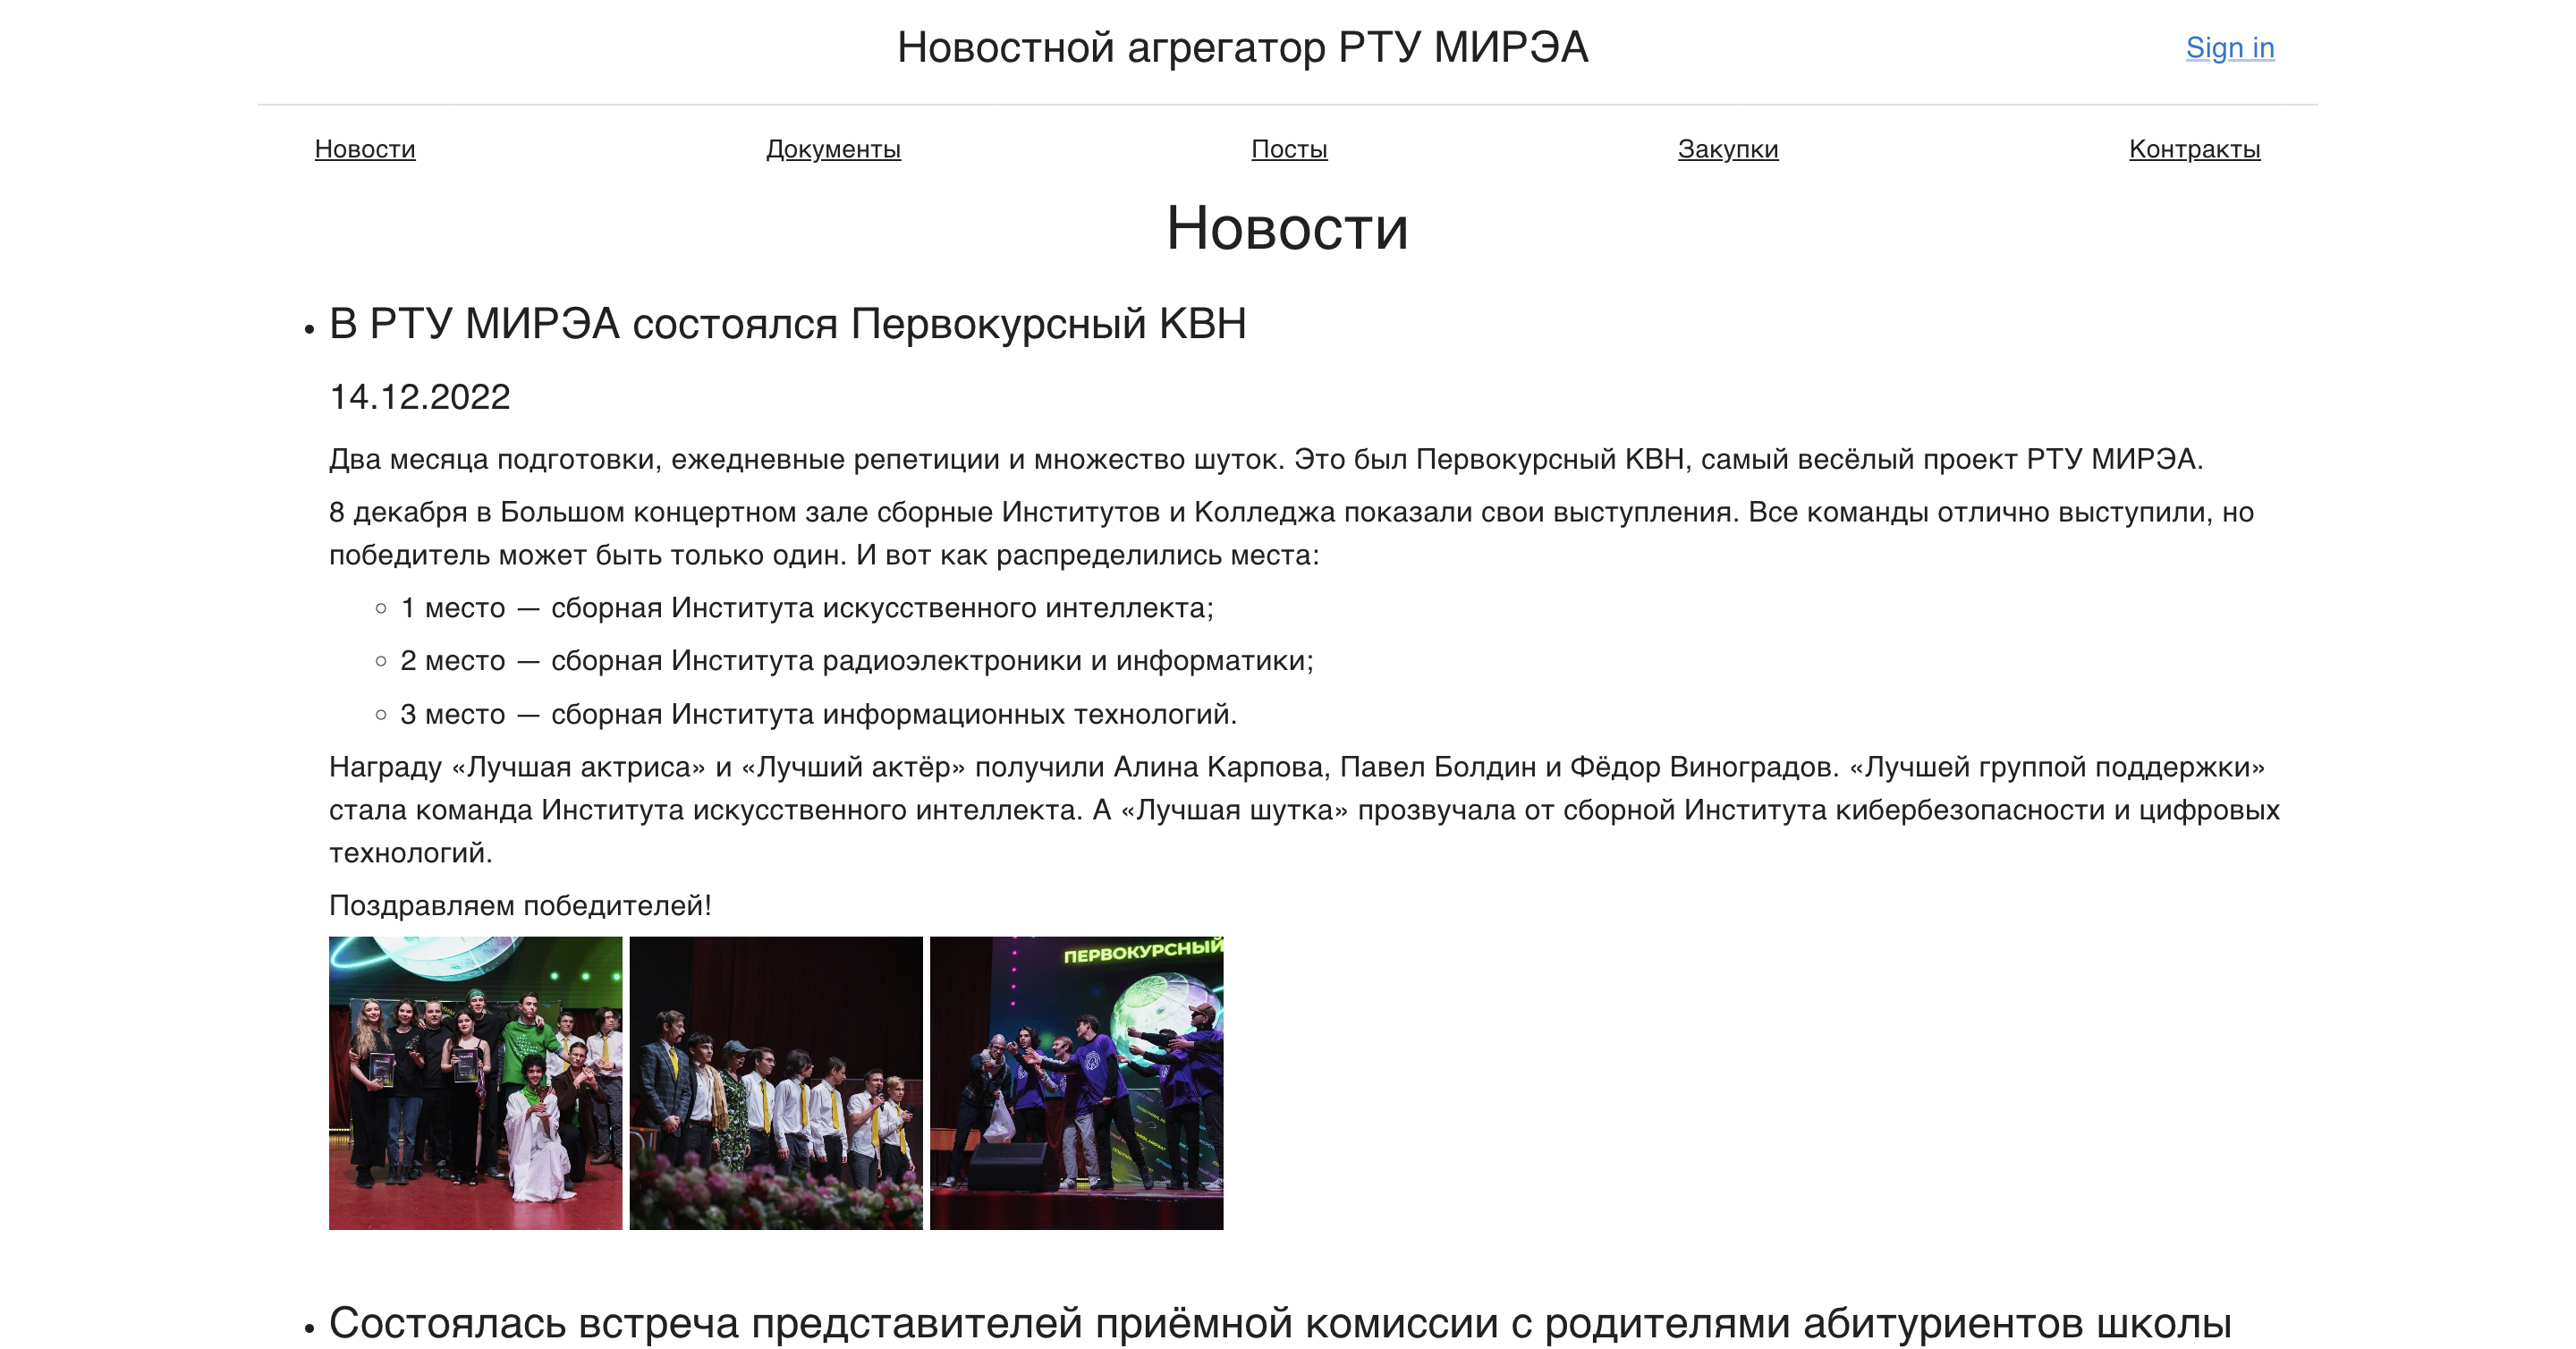
\includegraphics[width=\textwidth]{screen_news}
		\parskip=6pt
		\caption{Новости РТУ МИРЭА}
		\label{fig:screen_news}
	\end{figure}

	\begin{figure}[H]
		\centering
		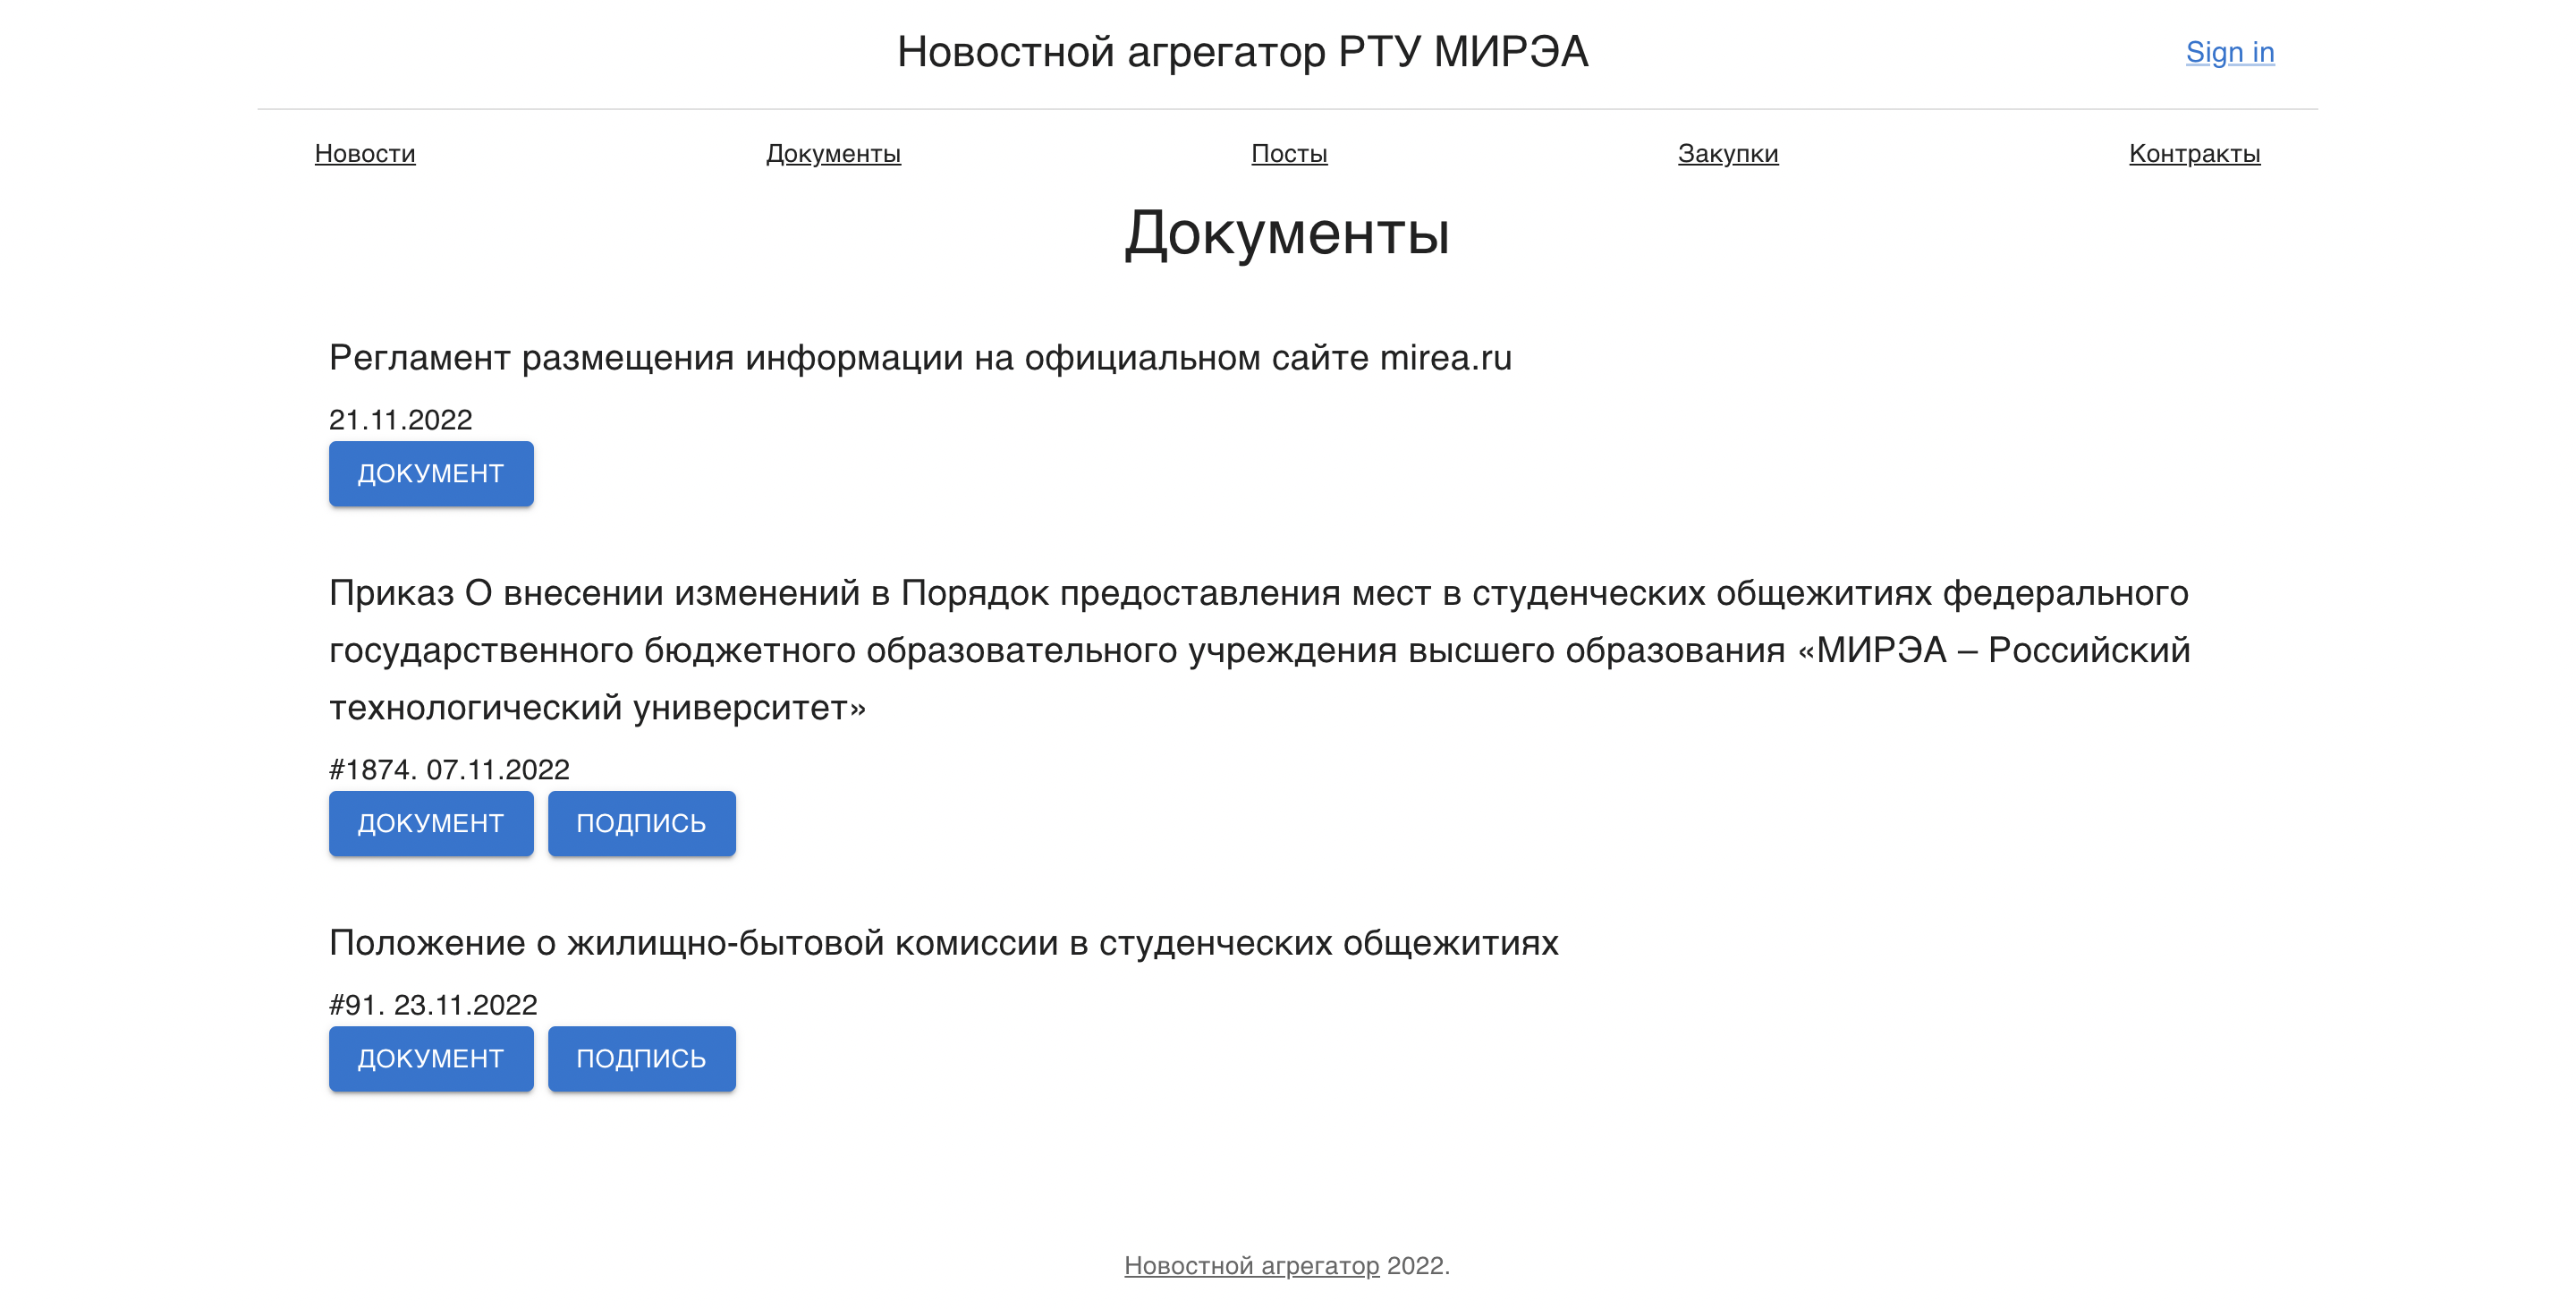
\includegraphics[width=\textwidth]{screen_docs}
		\parskip=6pt
		\caption{Документы РТУ МИРЭА}
	\end{figure}

	\begin{figure}[H]
		\centering
		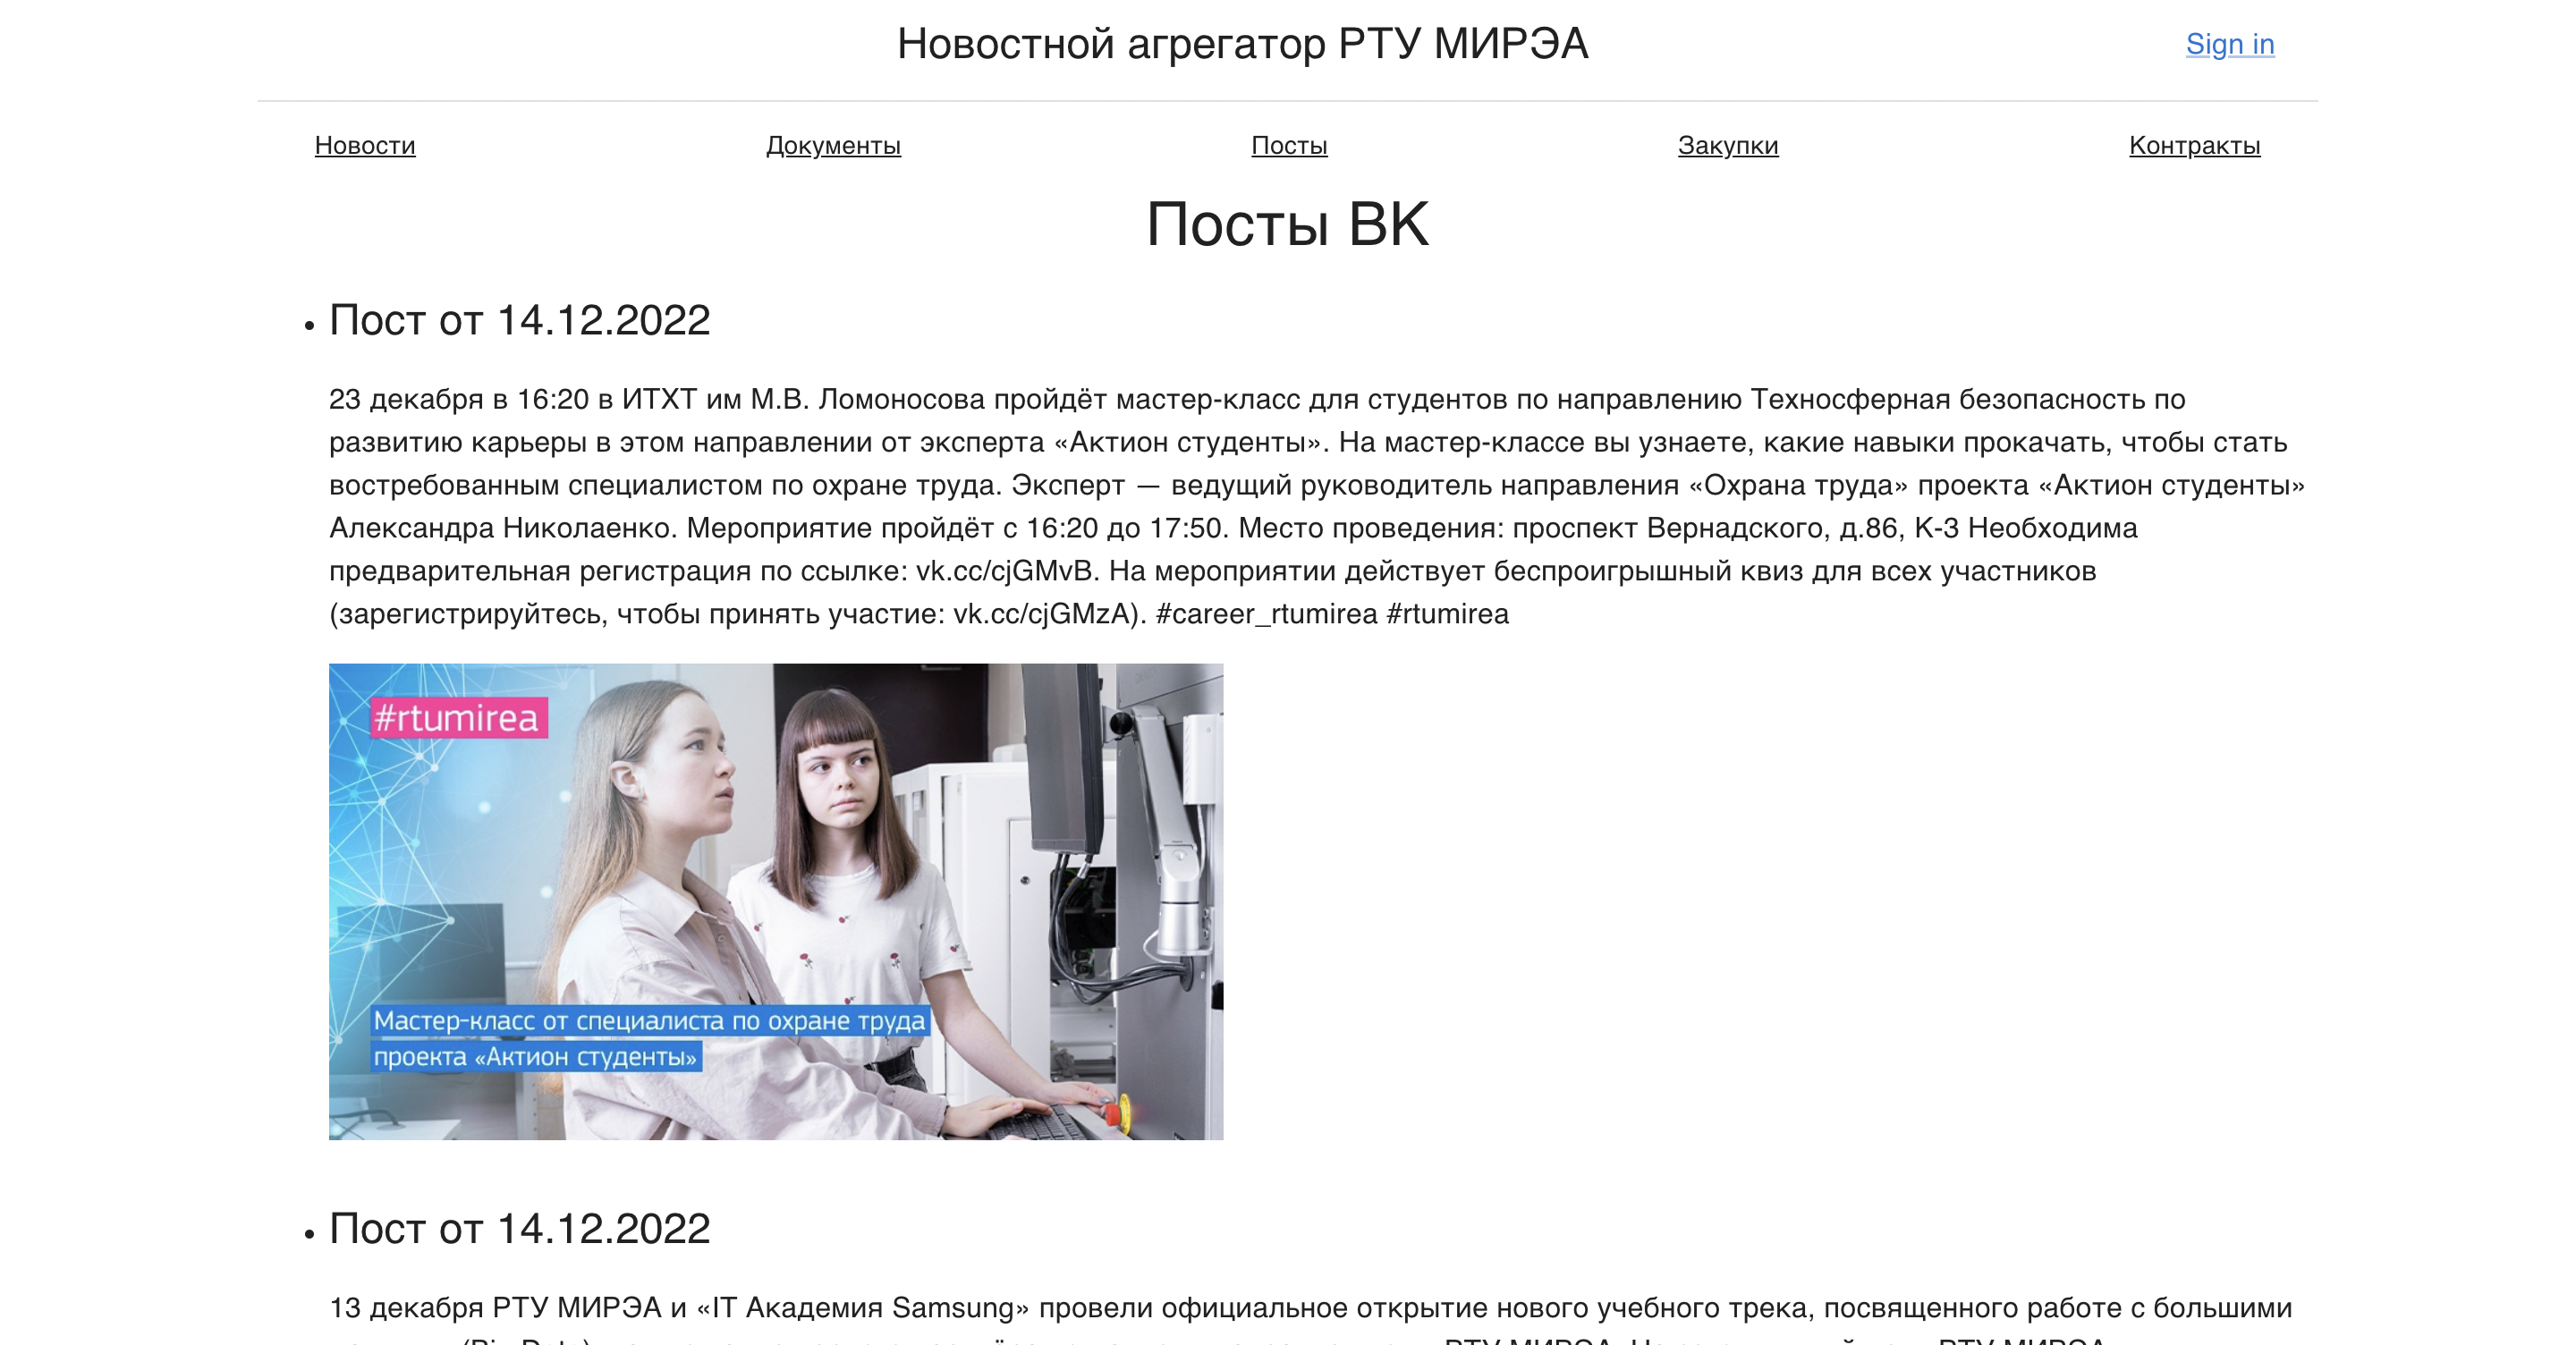
\includegraphics[width=\textwidth]{screen_posts}
		\parskip=6pt
		\caption{Посты РТУ МИРЭА}
	\end{figure}

	\begin{figure}[H]
		\centering
		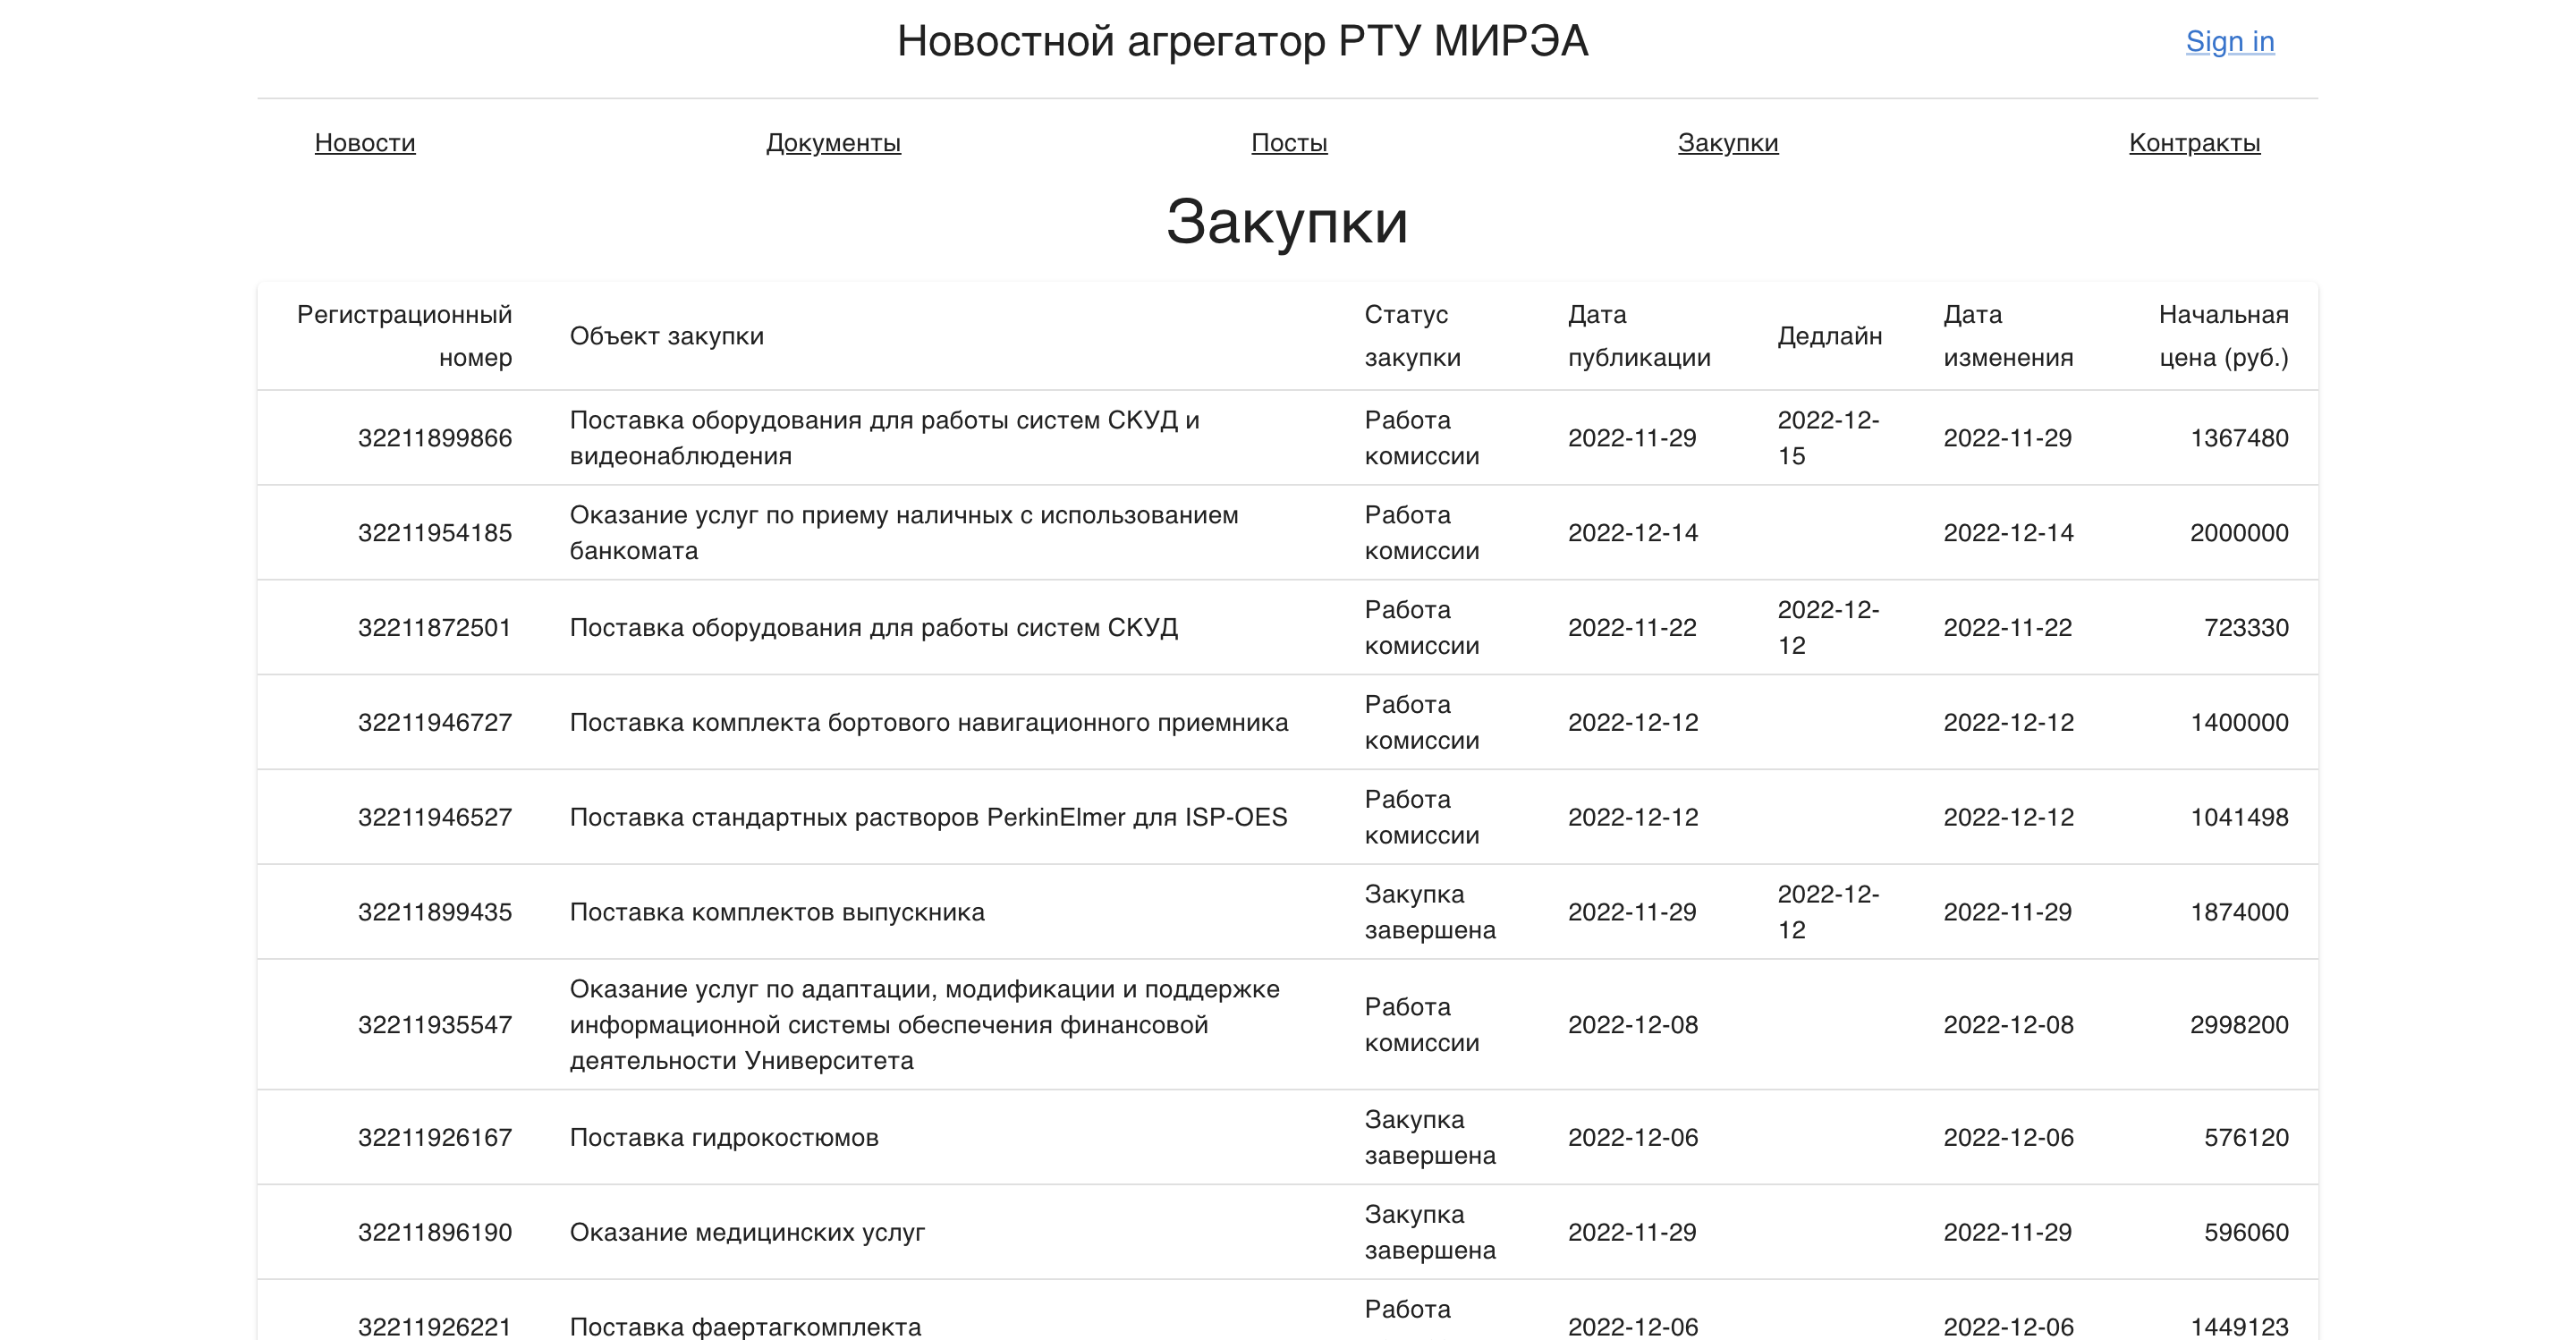
\includegraphics[width=\textwidth]{screen_purchases}
		\parskip=6pt
		\caption{Закупки РТУ МИРЭА}
	\end{figure}

	\begin{figure}[H]
		\centering
		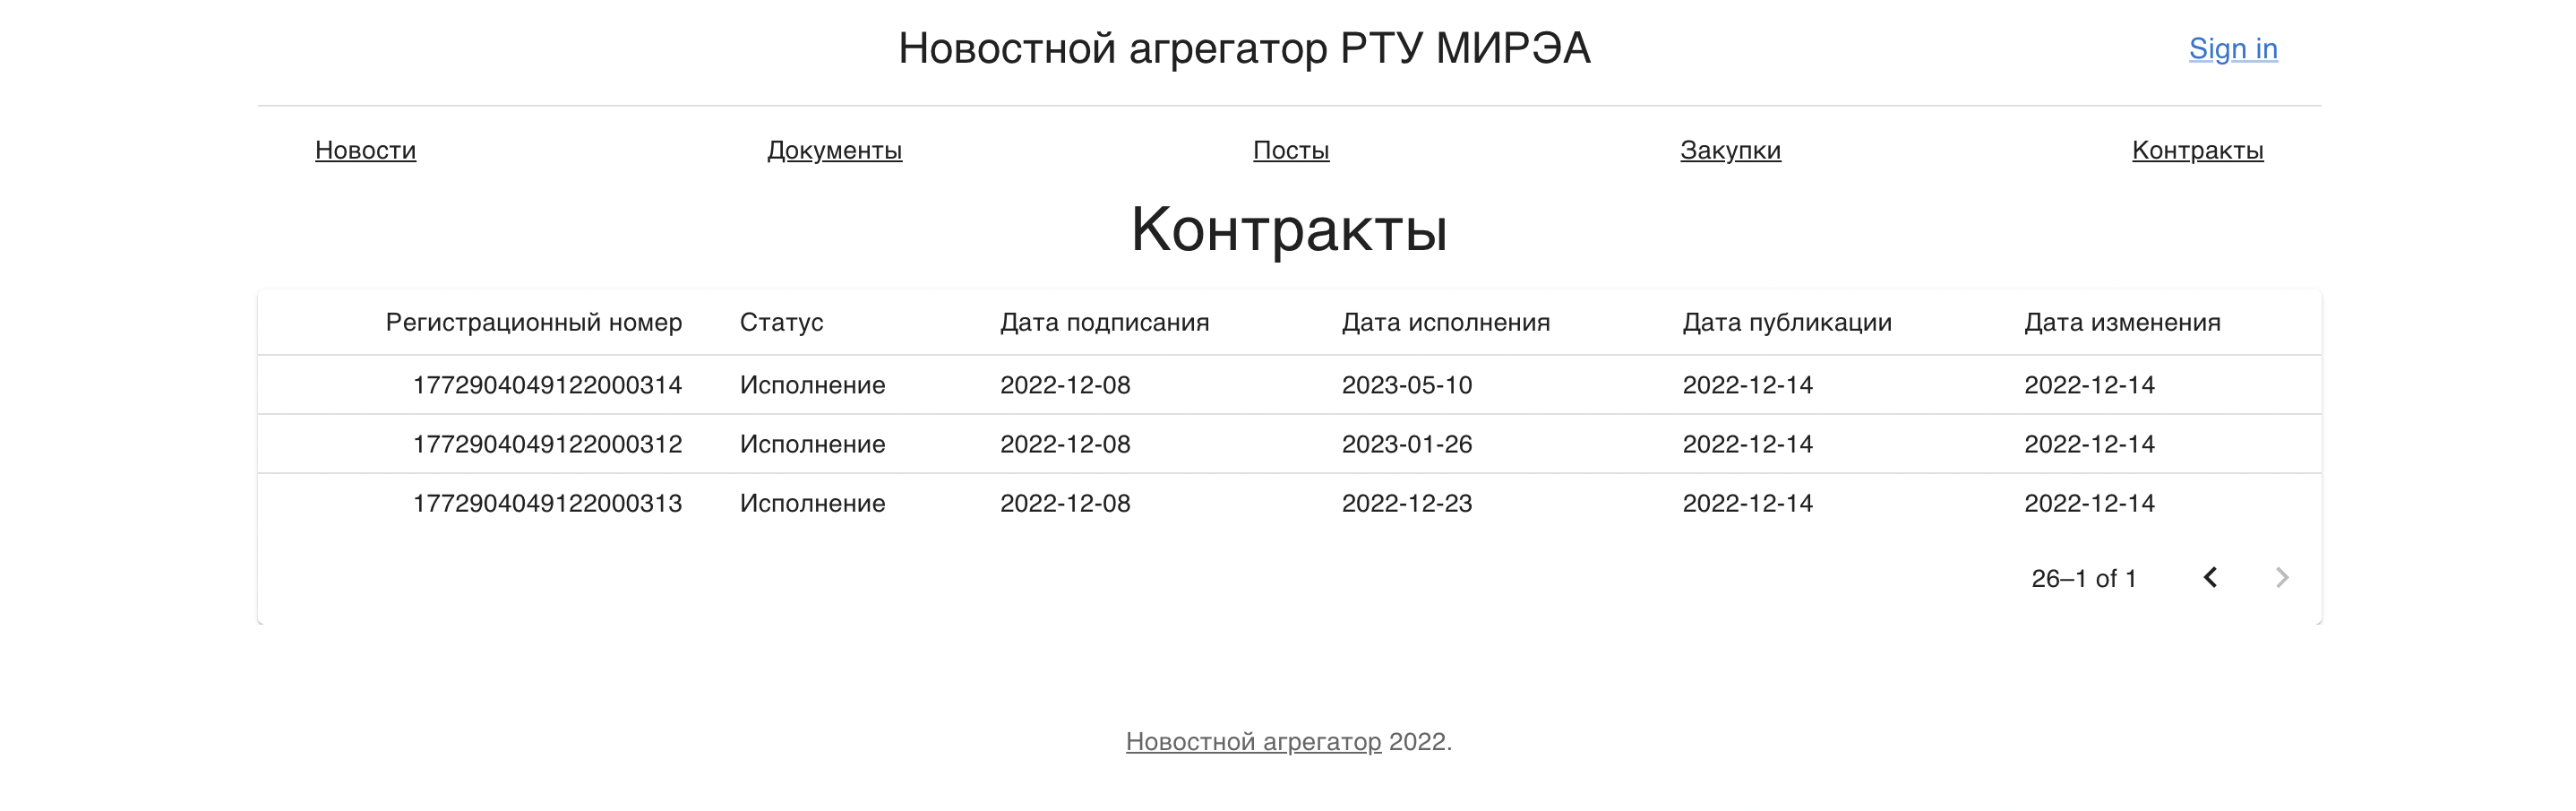
\includegraphics[width=\textwidth]{screen_contracts}
		\parskip=6pt
		\caption{Контракты РТУ МИРЭА}
	\end{figure}
	
	\subsection{Таблицы и сущности}
	
	На рисунках \ref{fig:full_mireanews}--\ref{fig:full_purchases} приведены примеры заполнения таблиц
	
	\begin{figure}[H]
		\centering
		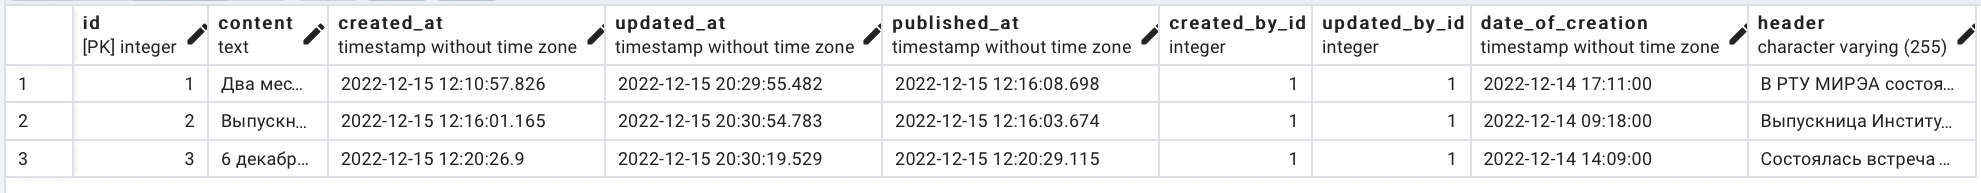
\includegraphics[width=\textwidth]{full_mireanews}
		\parskip=6pt
		\caption{Новости РТУ МИРЭА}
		\label{fig:full_mireanews}
	\end{figure}

	\begin{figure}[H]
		\centering
		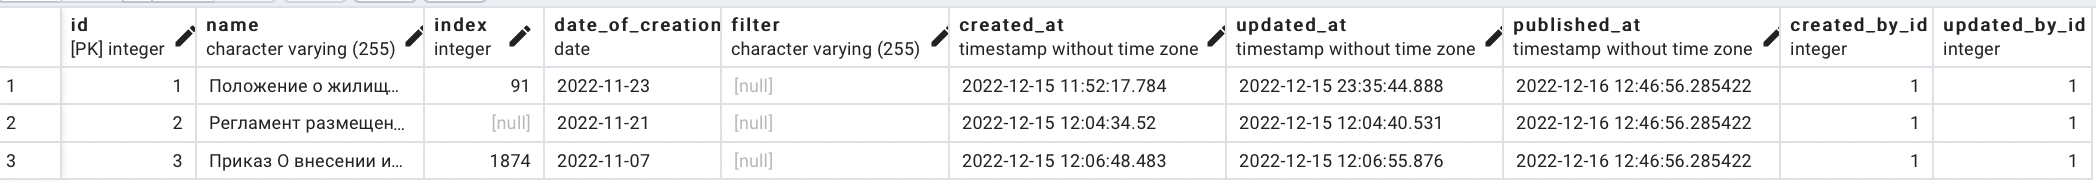
\includegraphics[width=\textwidth]{full_mireadocs}
		\parskip=6pt
		\caption{Документы РТУ МИРЭА}
	\end{figure}

	\begin{figure}[H]
		\centering
		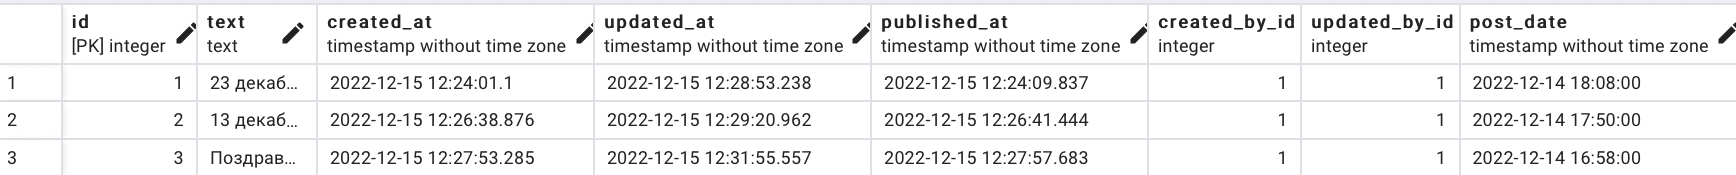
\includegraphics[width=\textwidth]{full_vkposts}
		\parskip=6pt
		\caption{Посты РТУ МИРЭА}
	\end{figure}

	\begin{figure}[H]
		\centering
		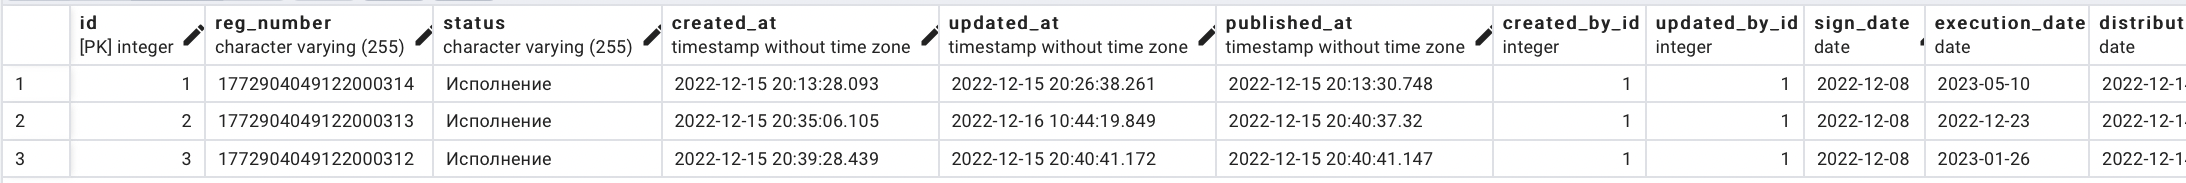
\includegraphics[width=\textwidth]{full_contracts}
		\parskip=6pt
		\caption{Контракты РТУ МИРЭА}
	\end{figure}

	\begin{figure}[H]
		\centering
		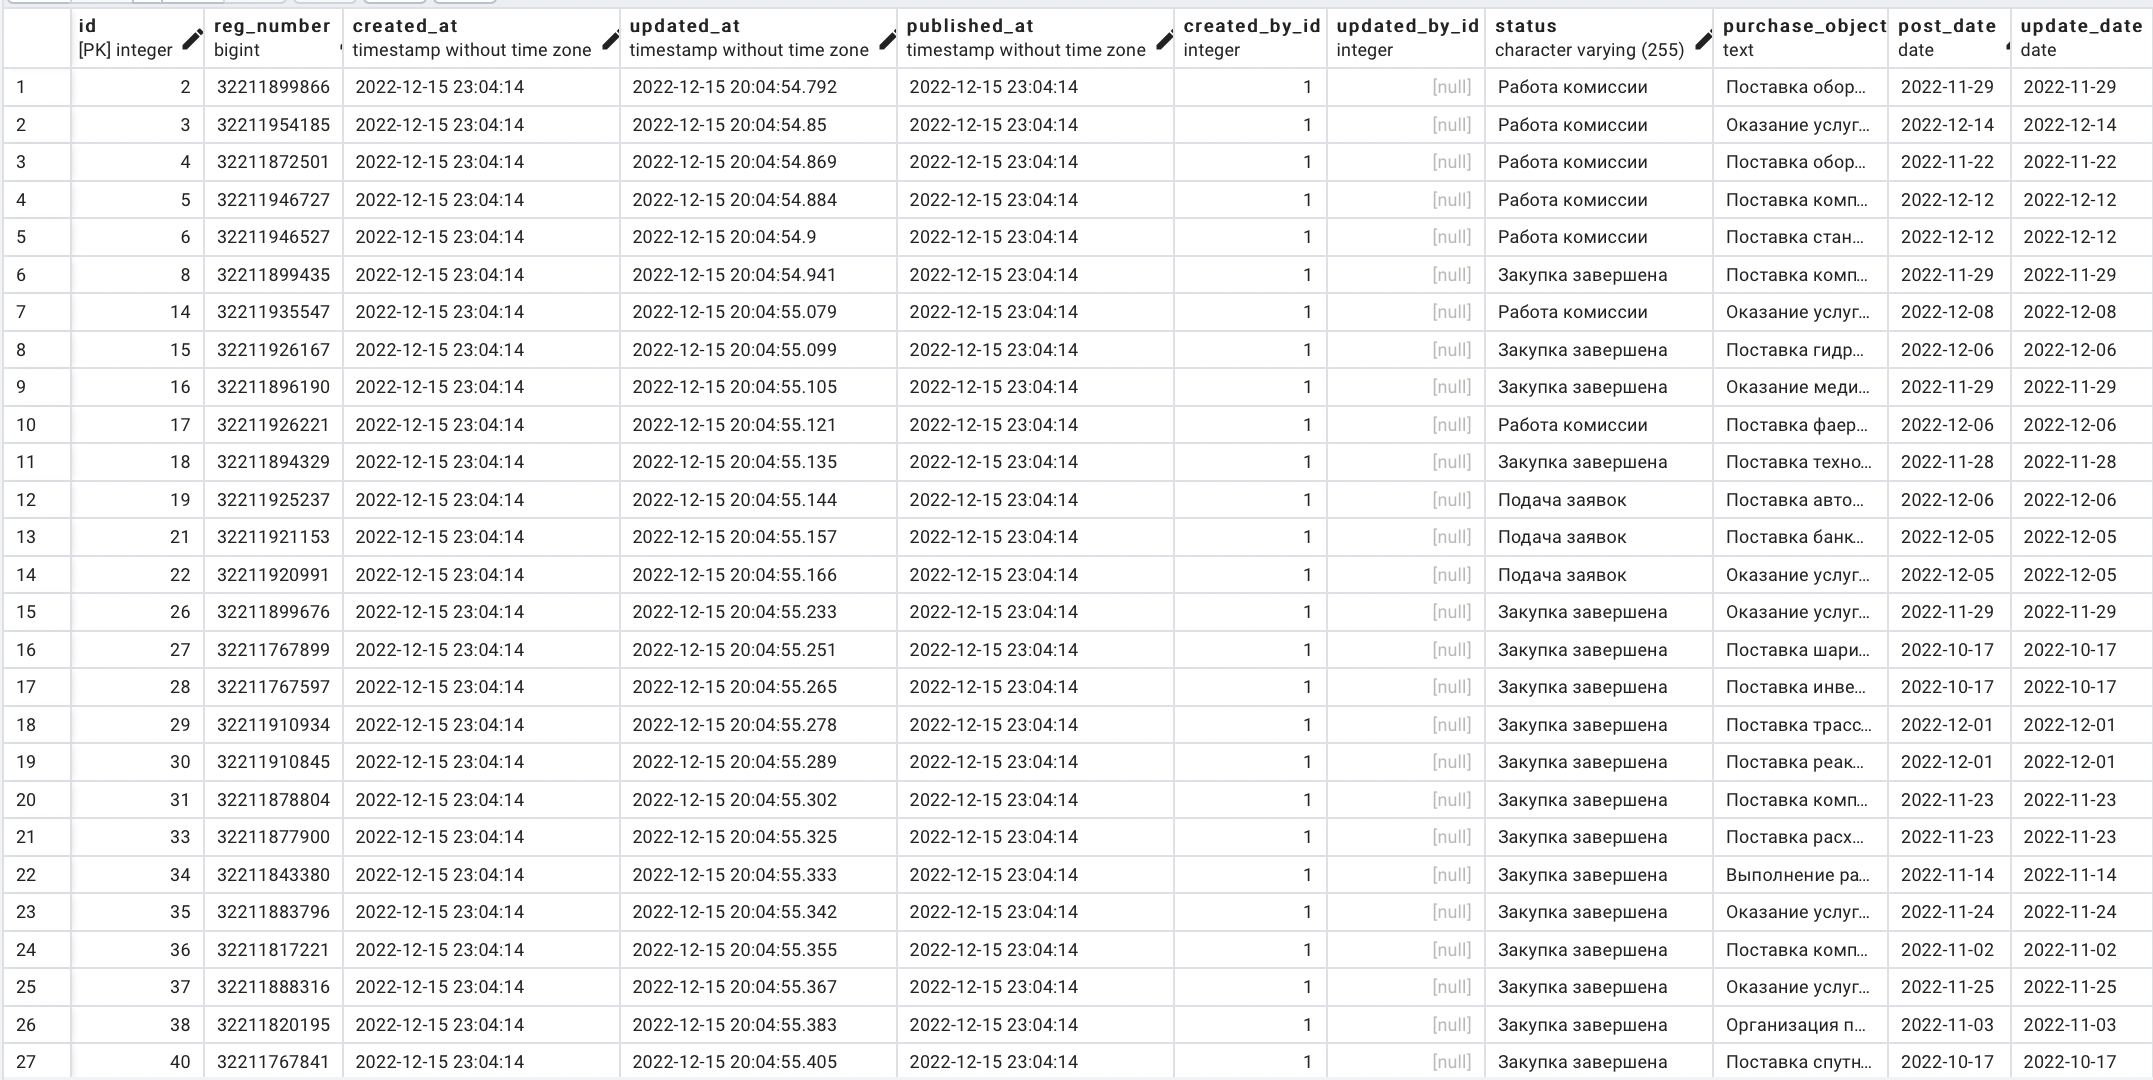
\includegraphics[width=\textwidth]{full_purchases}
		\parskip=6pt
		\caption{Закупки РТУ МИРЭА}
		\label{fig:full_purchases}
	\end{figure}
	
	
	\subsection{Оформление работы}
	
	Для написания пояснительной записки создан \LaTeX{} 2e класс документа, доступный по ссылке с примерами \url{https://github.com/mirea-ninja/Latex-Template-for-Report-Diploma-Thesis/}.
	
	
	\section*{Заключение}
	\phantomsection
	\addcontentsline{toc}{section}{Заключение}
	
	В рамках данного курсового проекта были выполнены следующие задачи:
	\begin{itemize}
		\item Анализ предметной области агрегатора новостей РТУ МИРЭА,
		\item Приобретение навыков по созданию запросов различных типов,
		\item Настройка CMS,
		\item Реализация веб-приложения.
	\end{itemize}
	

	С помощью данной системы автоматизированы некоторые функции и в перспективе могут быть реализованы и многие другие, которые подразумевает база данных, но которые не добавлены в графический интерфейс, создание автоматизированных брокеров для парсинга.
	
	
	
	\begin{thebibliography}{99\kern\bibindent}
		\bibitem{bib:stounz} Стоунз PostgreSQL. Основы / Стоунз, Мэттью Ричард; , Нейл.~---
		М.: СПб:Символ-Плюс, 2002.~--- 640 c.
		\bibitem{bib:postgrespro} PostgreSQL: Документация [Электронный ресурс] / URL:
		\url{https://postgrespro.ru/docs/postgresql} (дата обращения: 20.12.2022).
		\bibitem{bib:about} About // PostgreSQL. [Электронный ресурс] / URL:
		\url{https://www.postgresql.org/about/} (дата обращения: 20.12.2021).
		\bibitem{bib:metanit} Введение в PostgreSQL // Metanit. [2012-2022] / URL:
		\url{https://metanit.com/sql/postgresql/1.1.php} (дата обращения: 20.12.2022).
		\bibitem{bib:uorlsy} Уорсли, Дж. PostgreSQL. Для профессионалов (+ CD) / Дж.
		Уорсли, Дж.Дрейк. - М.: СПб: Питер, 2002.~--- 496 c.
	\end{thebibliography}
	
	
	
	
\end{document}
